
\section{Introduction}


Dynamic programming languages, with the exception of Perl, have surpassed compiled programming languages in terms of popularity among software system developers over the past decade (cf. Figure~\ref{fig:pypl}).
However, it remains unclear whether this category of dynamic programming languages can truly compete with compiled ones in terms of power consumption.
\begin{figure}[htbp]
    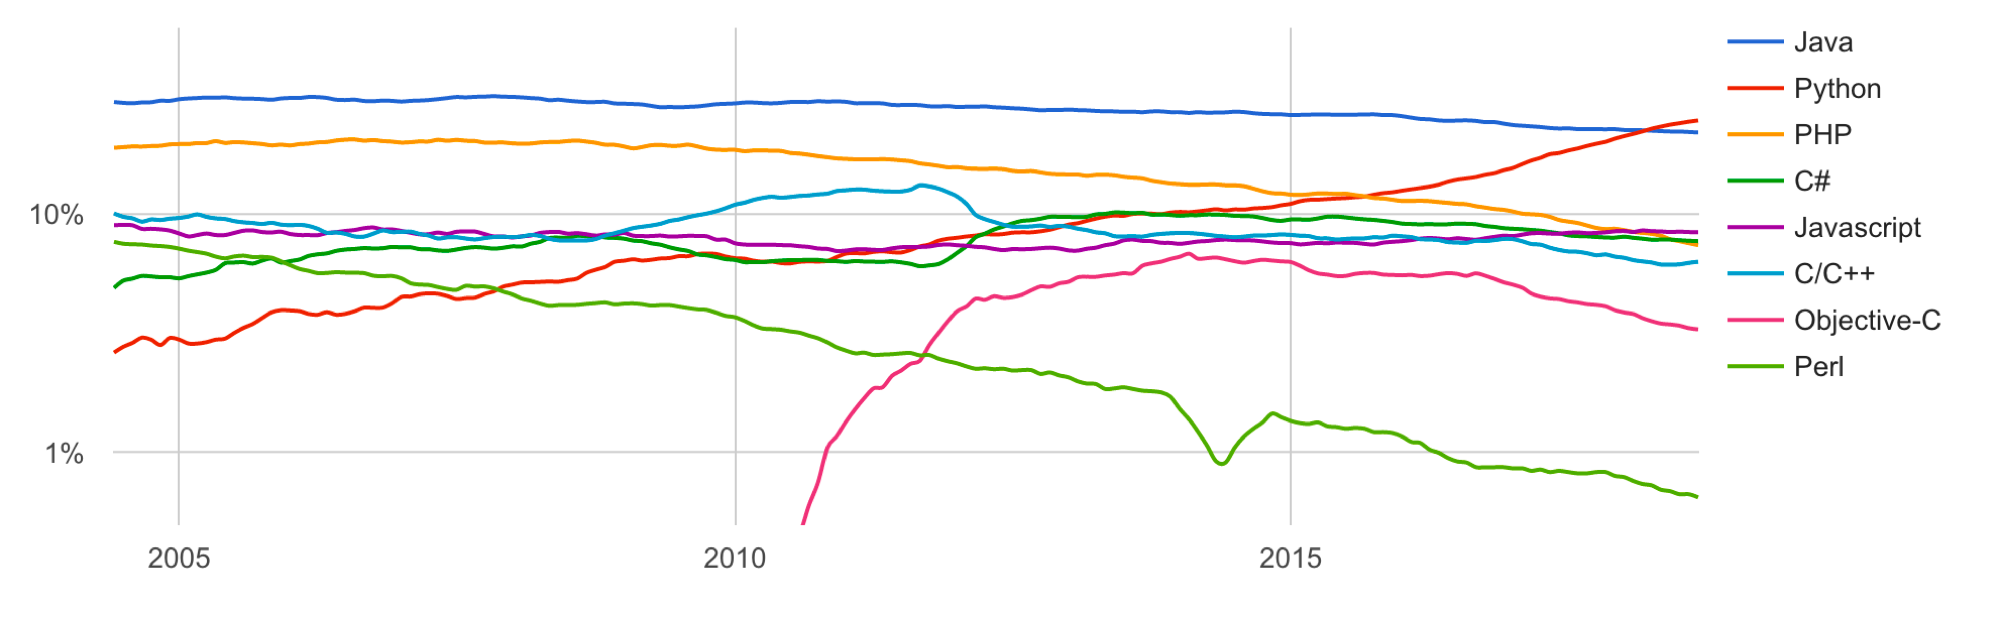
\includegraphics[width=\linewidth]{imgs/programminglanguangespopularity.png}
    \caption{PYPL Popularity of Programming Languages~\cite{noauthor_pypl_nodate}}
    \label{fig:pypl}
\end{figure}

In particular, Noureddine~\emph{et~al.}~\cite{noureddine_preliminary_2012} in 2012, and then Pereira~\emph{et~al.}~\cite{pereira_energy_2017} in 2017, conducted empirical power measurements on this topic, and both concluded that compiled programming languages overcome dynamic ones when it comes to power consumption.
According to their experiments, an interpreted programming language like Python can impose up to a $7,588\,\%$ energy overhead compared to C~\cite{pereira_energy_2017} (cf. Figure~\ref{fig:hannoi}).
In this chapter, we therefore explore the oblivious optimizations that can be applied to Python legacy applications in order to reduce their energy footprint.
As Python is widely adopted by software services deployed in public and private Cloud infrastructures, we believe that our contributions will benefit to wide diversity of legacy systems and not only favorably contribute to reduce the carbon emissions of ICT, but also reduce their cloud invoice for the resources consumed by these services.
More specifically, this chapter focuses on runtime optimizations that can adopted by developers to leverage the power consumption of Python applications.
We start by studuing the impact of some of programmers choice such as the type of data structures or loops, on the global energy consumption of the execution code.
then we discuss some other factors such as level of concurrency etc. later we we will talk about another non intrusive ways to optimize the energy consumption of this code. one kind of those optimizations includes alternative interpertersand some libraries that are dedicated to optimize the code without changing its structures such as \emph{ahead-of-time} (AOT) compilation and \emph{just-in-time} (JIT) libraries that are maintained by the community.

%%%%%%%%%%% READ AGAIN 
% articular, Noureddine in 2012 and Pereira in 2017 conducted empirical power measurements on this topic, and both concluded that compiled programming languages consume less power than dynamic ones.They found that a programming language that is interpreted, like Python, can use up to 7,584 times more energy than C. As a result, in this chapter, we will look at the obvious optimizations that may be done to Python legacy programs to lower their energy footprint.Since Python is used by many software services in both public and private cloud infrastructures, we think that our contributions will help a wide range of legacy systems by reducing ICT carbon emissions and lowering cloud bills for the resources used by these services. This chapter focuses on runtime improvements that developers can employ to reduce the power consumption of Python applications.We start by looking at how the choices made by programmers, like the type of data structure or loop, affect how much energy the code as a whole uses. Then we discuss additional topics, such as the level of concurrency, and so on.We will discuss another non-intrusive technique to optimize this code's energy consumption.Alternative interpreters and libraries dedicated to optimizing code without affecting its structures, such as ahead-of-time (AOT) compilation and just-in-time (JIT) libraries maintained by the community, are examples of these optimizations. 
% However, the operational conditions under which these measurements may threaten the validity of their results.



\section{Motivation}
\subsection{python popularity}

Nowadays, Python seems to attract a large community of developers who are interested in data analysis, web development, system administration, and machine learning—according to a survey conducted in 2018 by JetBrains ---\footnote{\url{https://www.jetbrains.com/research/python-developers-survey-2018/}}one can fear that the wide adoption of dynamic programming languages, like Python, in production may critically hamper the power consumption of ICT.
As the popularity of such dynamic programming languages partly builds on the wealth and the diversity of their ecosystem (\emph{e.g.}, the NumPY, SciKit\,Learn, and Panda libraries in Python), one cannot reasonably expect that developers will likely move to an alternative programming language mostly for energy considerations.
Rather, we believe that a better option consists of leveraging the strength of this rich ecosystem to promote energy-efficient solutions in order to improve the power consumption of legacy software systems.




% The contributions of this chapter can therefore be summarized as:
% \begin{compactenum}
%     \item a classification of state-of-the-art Python optimizations,
%     \item an evaluation of the power efficiency of these optimizations on well-known micro-benchmarks,
%     \item a comparison of the effective energy efficiency of Python compared to compiled languages,
%     \item an assessment of the energy speedup of these optimizations on representative applications and workloads.
% \end{compactenum}



\subsection{python gluttony}

In the other hand,because of the interpreted nature of Python code, this programming language has paid a high price in terms of performance.  \ref{fig:clbg}, memory and energy consumption.

\begin{figure}[htbp]
    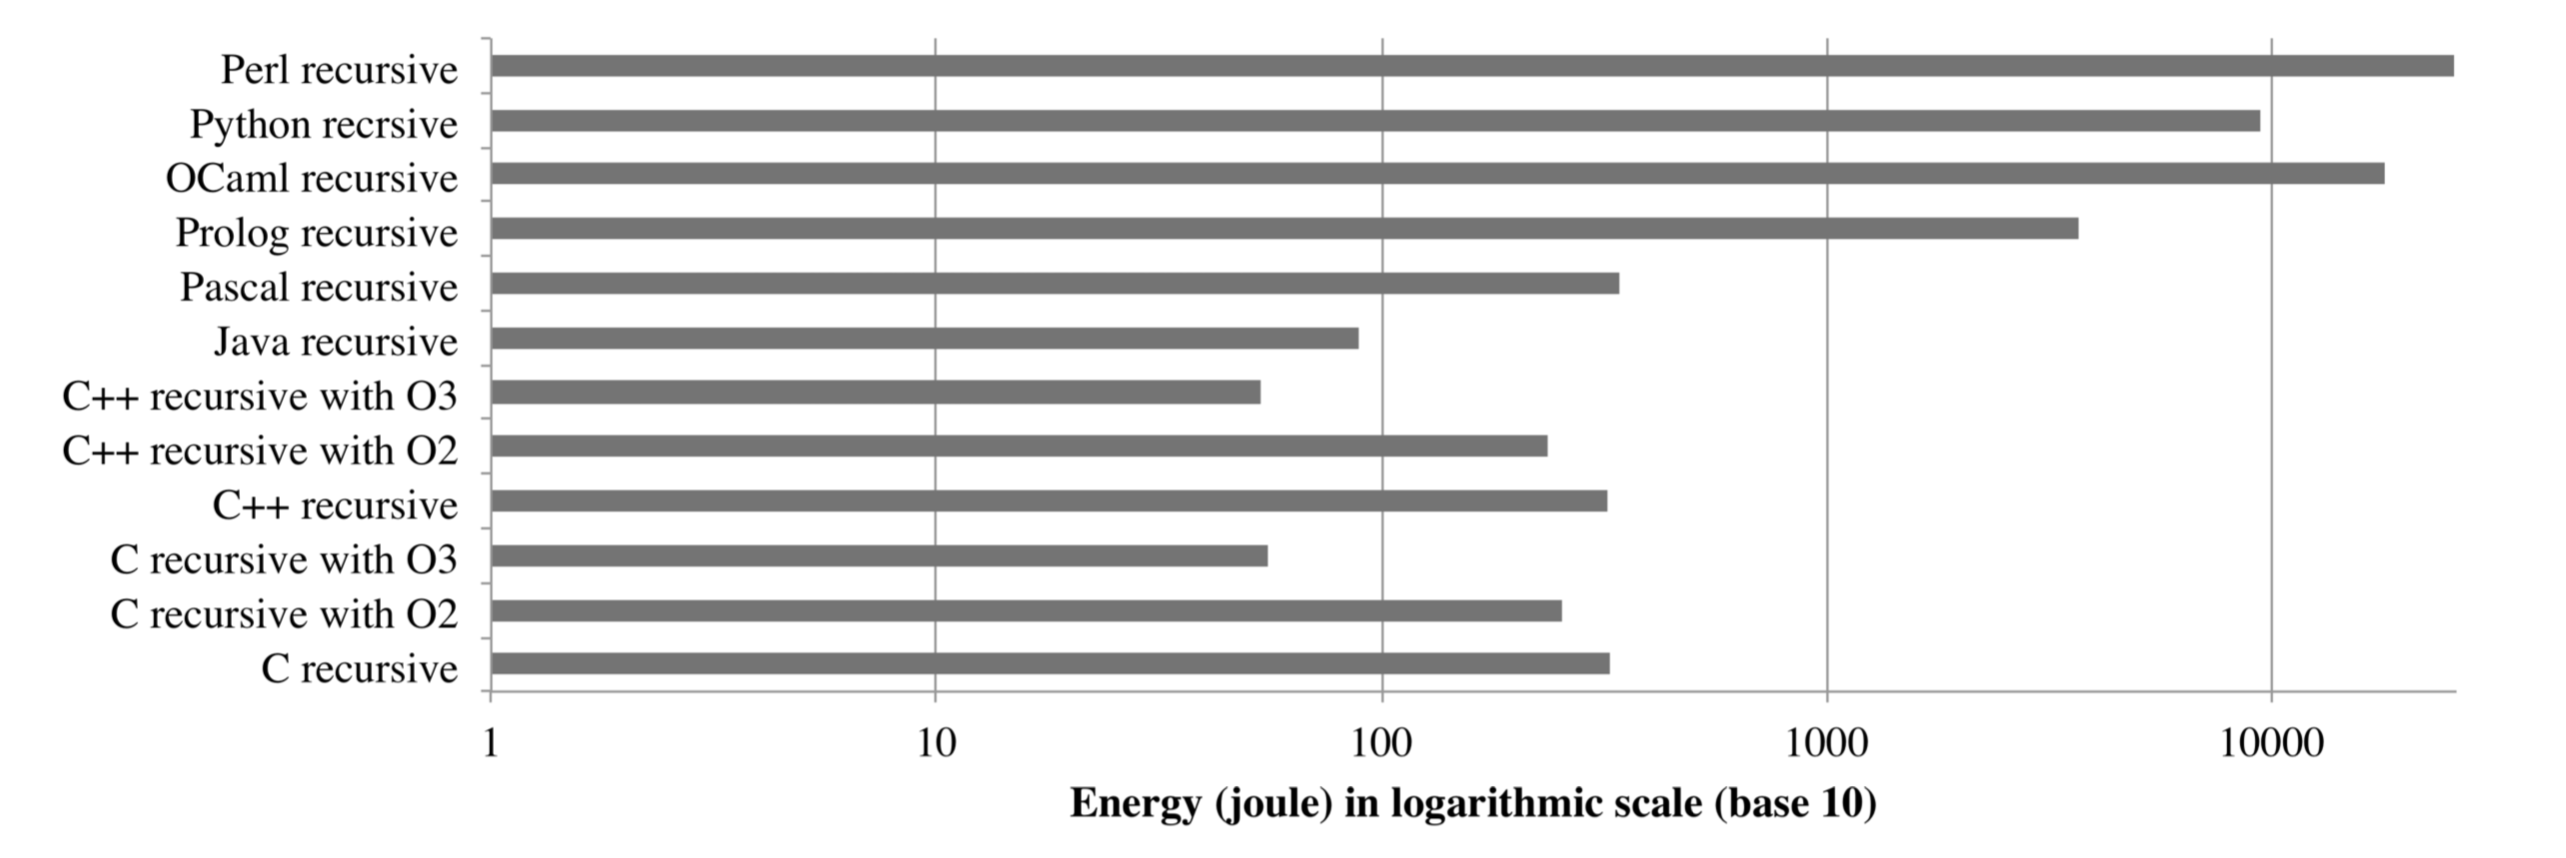
\includegraphics[width=\linewidth]{imgs/hannoiimplementation.png}
    \caption{Energy consumption of a recursive implementation of Tower of Hanoi program in different languages~\cite{noureddine_preliminary_2012}}
    \label{fig:hannoi}
\end{figure}

According to \cite{pinto_energy_2017} and \cite{noureddine_preliminary_2012}, Python tends to be one more energy hungry . As onne can notice in figure \ref{fig:hannoi}, python consumes 30 times more than C or C++. The test was done on an implementation of \fnurl{hannoi test}{ https://en.wikipedia.org/wiki/Tower_of_Hanoi}  30 disks.

Python consumes a lot of energy, mainly because it is slow in execution. Its flexibility and simplicity caused it to drop off in performance, because Python gains its flexibility from being a dynamic language. Therefore, it needs an interpreter to execute its programs, which makes them much slower compared to the others that are written in compiled programming languages such as C and C++ or semi-compiled languages like Java.

As shown in Table\ref{fig:clbg}, one can see that in most of the test cases, Python takes more time to execute-the only case that he wasn't the last one was in the benchmark regx-redux where he beat Go-, and in some cases the gap was huge, such as in the n-body test where Python took around 100 times more than C++.\footnote{\url{https://benchmarksgame-team.pages.debian.net/benchmarksgame/index.html}}
\begin{table}[hbt]
    \begin{tabular}{l|*{5}c}
                           & C    & C++   & Java & python & Go    \\
        \hline
        pidigits           & 1.75 & 1.89  & 3.13 & 3.51   & 2.04  \\
        reverse-complement & 1.75 & 2.95  & 3.31 & 16.76  & 4.00  \\
        regx-redux         & 1.45 & 1.66  & 10.5 & 15.56  & 28.69 \\
        k-nucleotide       & 5.07 & 3.66  & 8.66 & 79.79  & 15.36 \\
        binary-trees       & 2.55 & 2.63  & 8.28 & 92.72  & 28.90 \\
        fasta              & 1.32 & 1.33  & 2.32 & 62.88  & 2.07  \\
        Fannkuch-redux     & 8.72 & 10.62 & 17.9 & 547.23 & 17.82 \\
        n-body             & 9.17 & 8.24  & 22.0 & 882.00 & 21.00 \\
        spectral-norm      & 1.99 & 1.98  & 4.27 & 193.86 & 3.95  \\
        Mandelbort         & 1.64 & 1.51  & 6.96 & 279.68 & 5.47  \\
    \end{tabular}
    \caption{Comparison of the execution time between different programming languages using the computer language benchmarks game}
    \label{fig:clbg}
\end{table}


\subsection{Goal}

To reduce the energy consumption of Python, we started by targeting the main usage of this programming language, which is revealed to be data science and web development. Figure~\ref{fig:usecase} illustrates a study made by the JetBrain company on Python developers. \footnote{\url{https://www.jetbrains.com/lp/python-developers-survey-2020}}.In this survey, multiple answers were accepted. As one can see, 57\% of the respondents said that they use Python for data science, 51\% said they are using it for web development, and around 40\% said they are using it for system administration.
\begin{figure}[hbt]
    \centering
    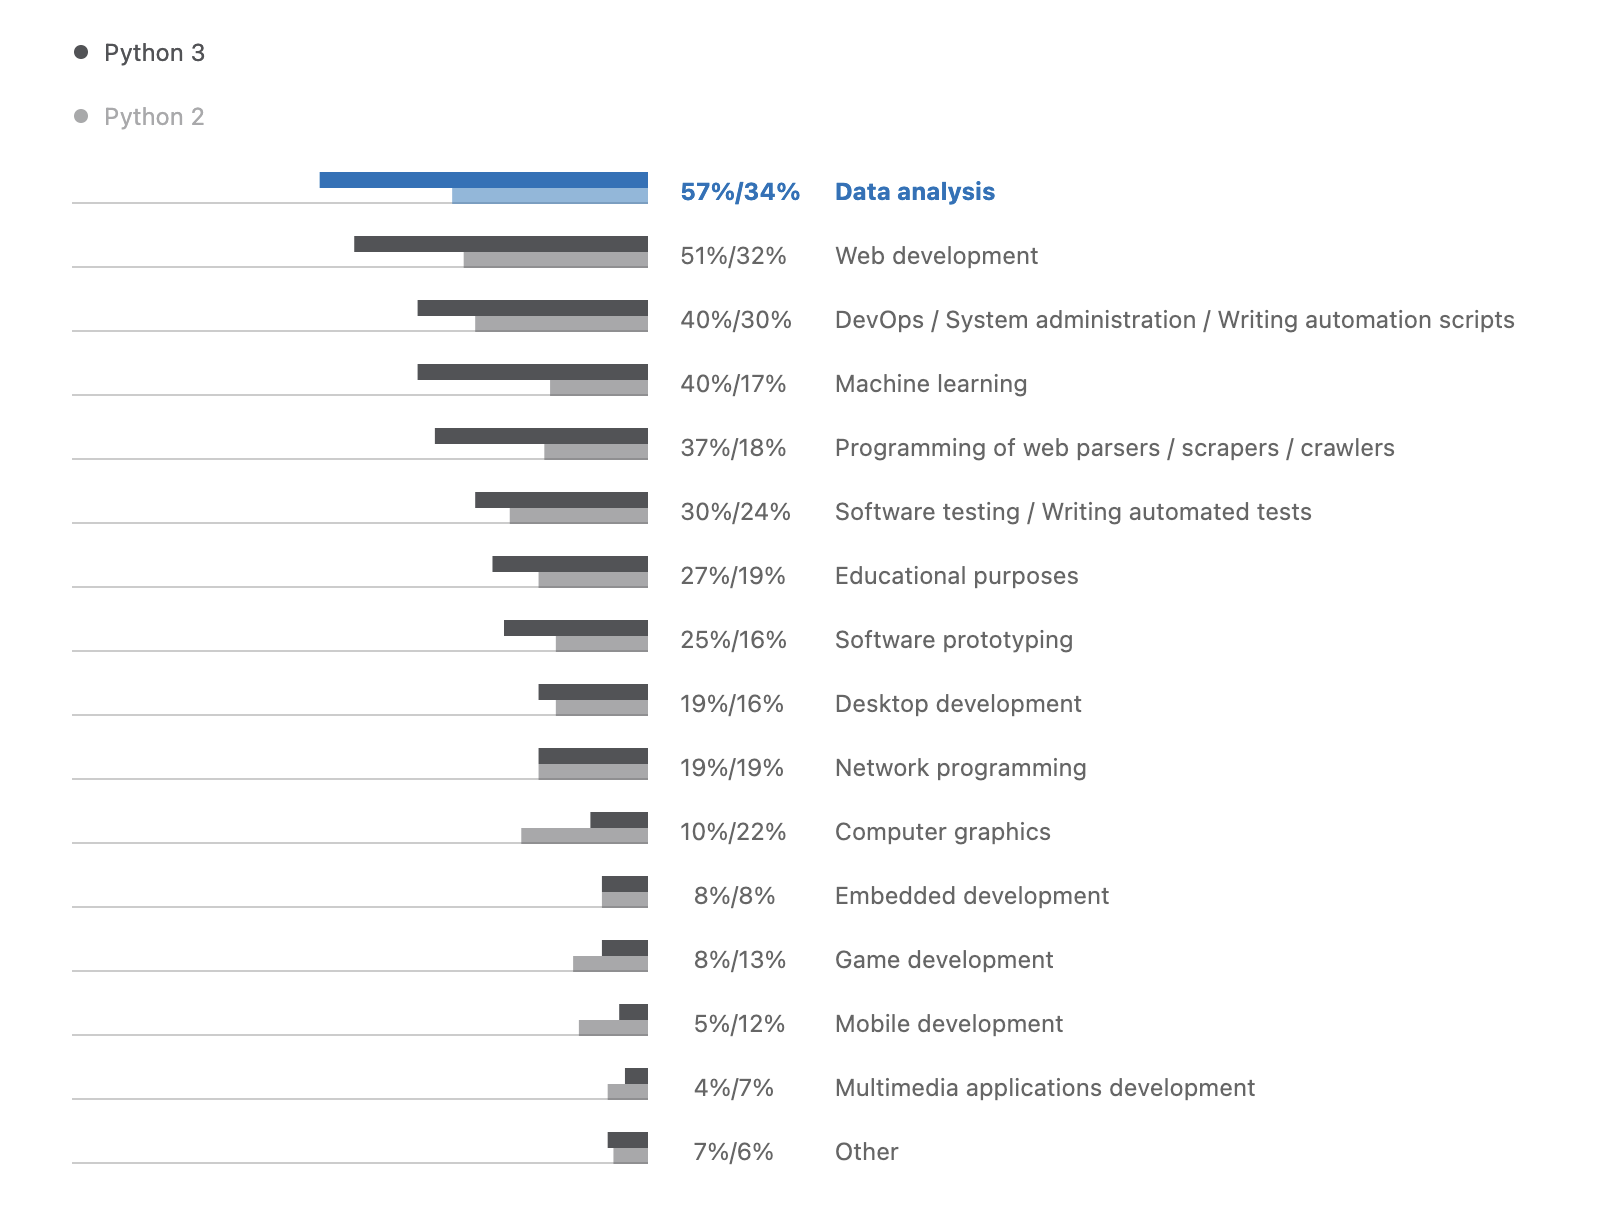
\includegraphics[width=\linewidth]{imgs/python_use_cases}
    \caption{Use cases of python }
    \label{fig:usecase}
\end{figure}

In this chapter, we will first investigate its behavior in the most common usage cases.Following that, we will focus on the language's structures in the hope of discovering some fundamental guidelines for more general purposes, as \citeauthor{hasan_energy_2016-1} did in their article~\cite{hasan_energy_2016-1}.
Following that, we will measure the energy consumption of several Python implementations in order to determine a non-intrusive technique to improve energy efficiency.

Therefore this chapter will target the following research questions :
\begin{compactenum}[\indent\bf RQ\,1:]
    \item \emph{What is the behavior of Python when it is used as a data science tool?}
    \item \emph{Are the default guidelines of Python energy efficient?}
    \item \emph{Can we reduce the energy consumption of Python programs without impacting the source code?}
\end{compactenum}




% \section{Experimental Protocol}\label{sec:pythonprotocol}
% In this section, we discuss the experimental setting, including hardware components, software components, and the methodology that we adopted to answer the previous research questions.
% For each of the questions that follow, we will first talk about how the experiment was done, and then we will talk about the results.


% %% should i include the part with the exceptions ??? naah no need so

% %% except the parallellism part , which i dont know how to link it here yet 
% \section{Workload} :
% for this chapter we are consediring 4 seperated, yet related studies .
% First we are going to see the energy behavriour of python within two study cases. Web servers and Machine learning. later we will dig deeper into the energy consumption of python basic structures where finally we will conclude with the impact of python interpterer on the energy consumption.




% \subsubsection{micro-benchmarks}

% \subsubsection{benchmarks}




\section{web developement}
first we wanted to test the energy consumption of python using on djagon,one of the most popular web frameworks.
therefore we create a simple website where we try to analyse the cost of a single request using different mechanisms to fetch the data from the database.
the idea behind this use case is to see wether the choice of the database and the orm ( object relational mapper) impacts the energy consumption and the perfromances of the website.

we considered using two different databases postgresSQL and SQlite3 that containes the same data, and three different ways to fetch the data.
\begin{enumerate}
    \item the naive version: which relies only on the ORM to get the data
    \item Prefetch : basically we just prefetch the data before we request it
    \item optimized : and here we optimize our request on the SQL level without passing by the ORM
\end{enumerate}

\begin{figure}[!hbt]
    \centering
    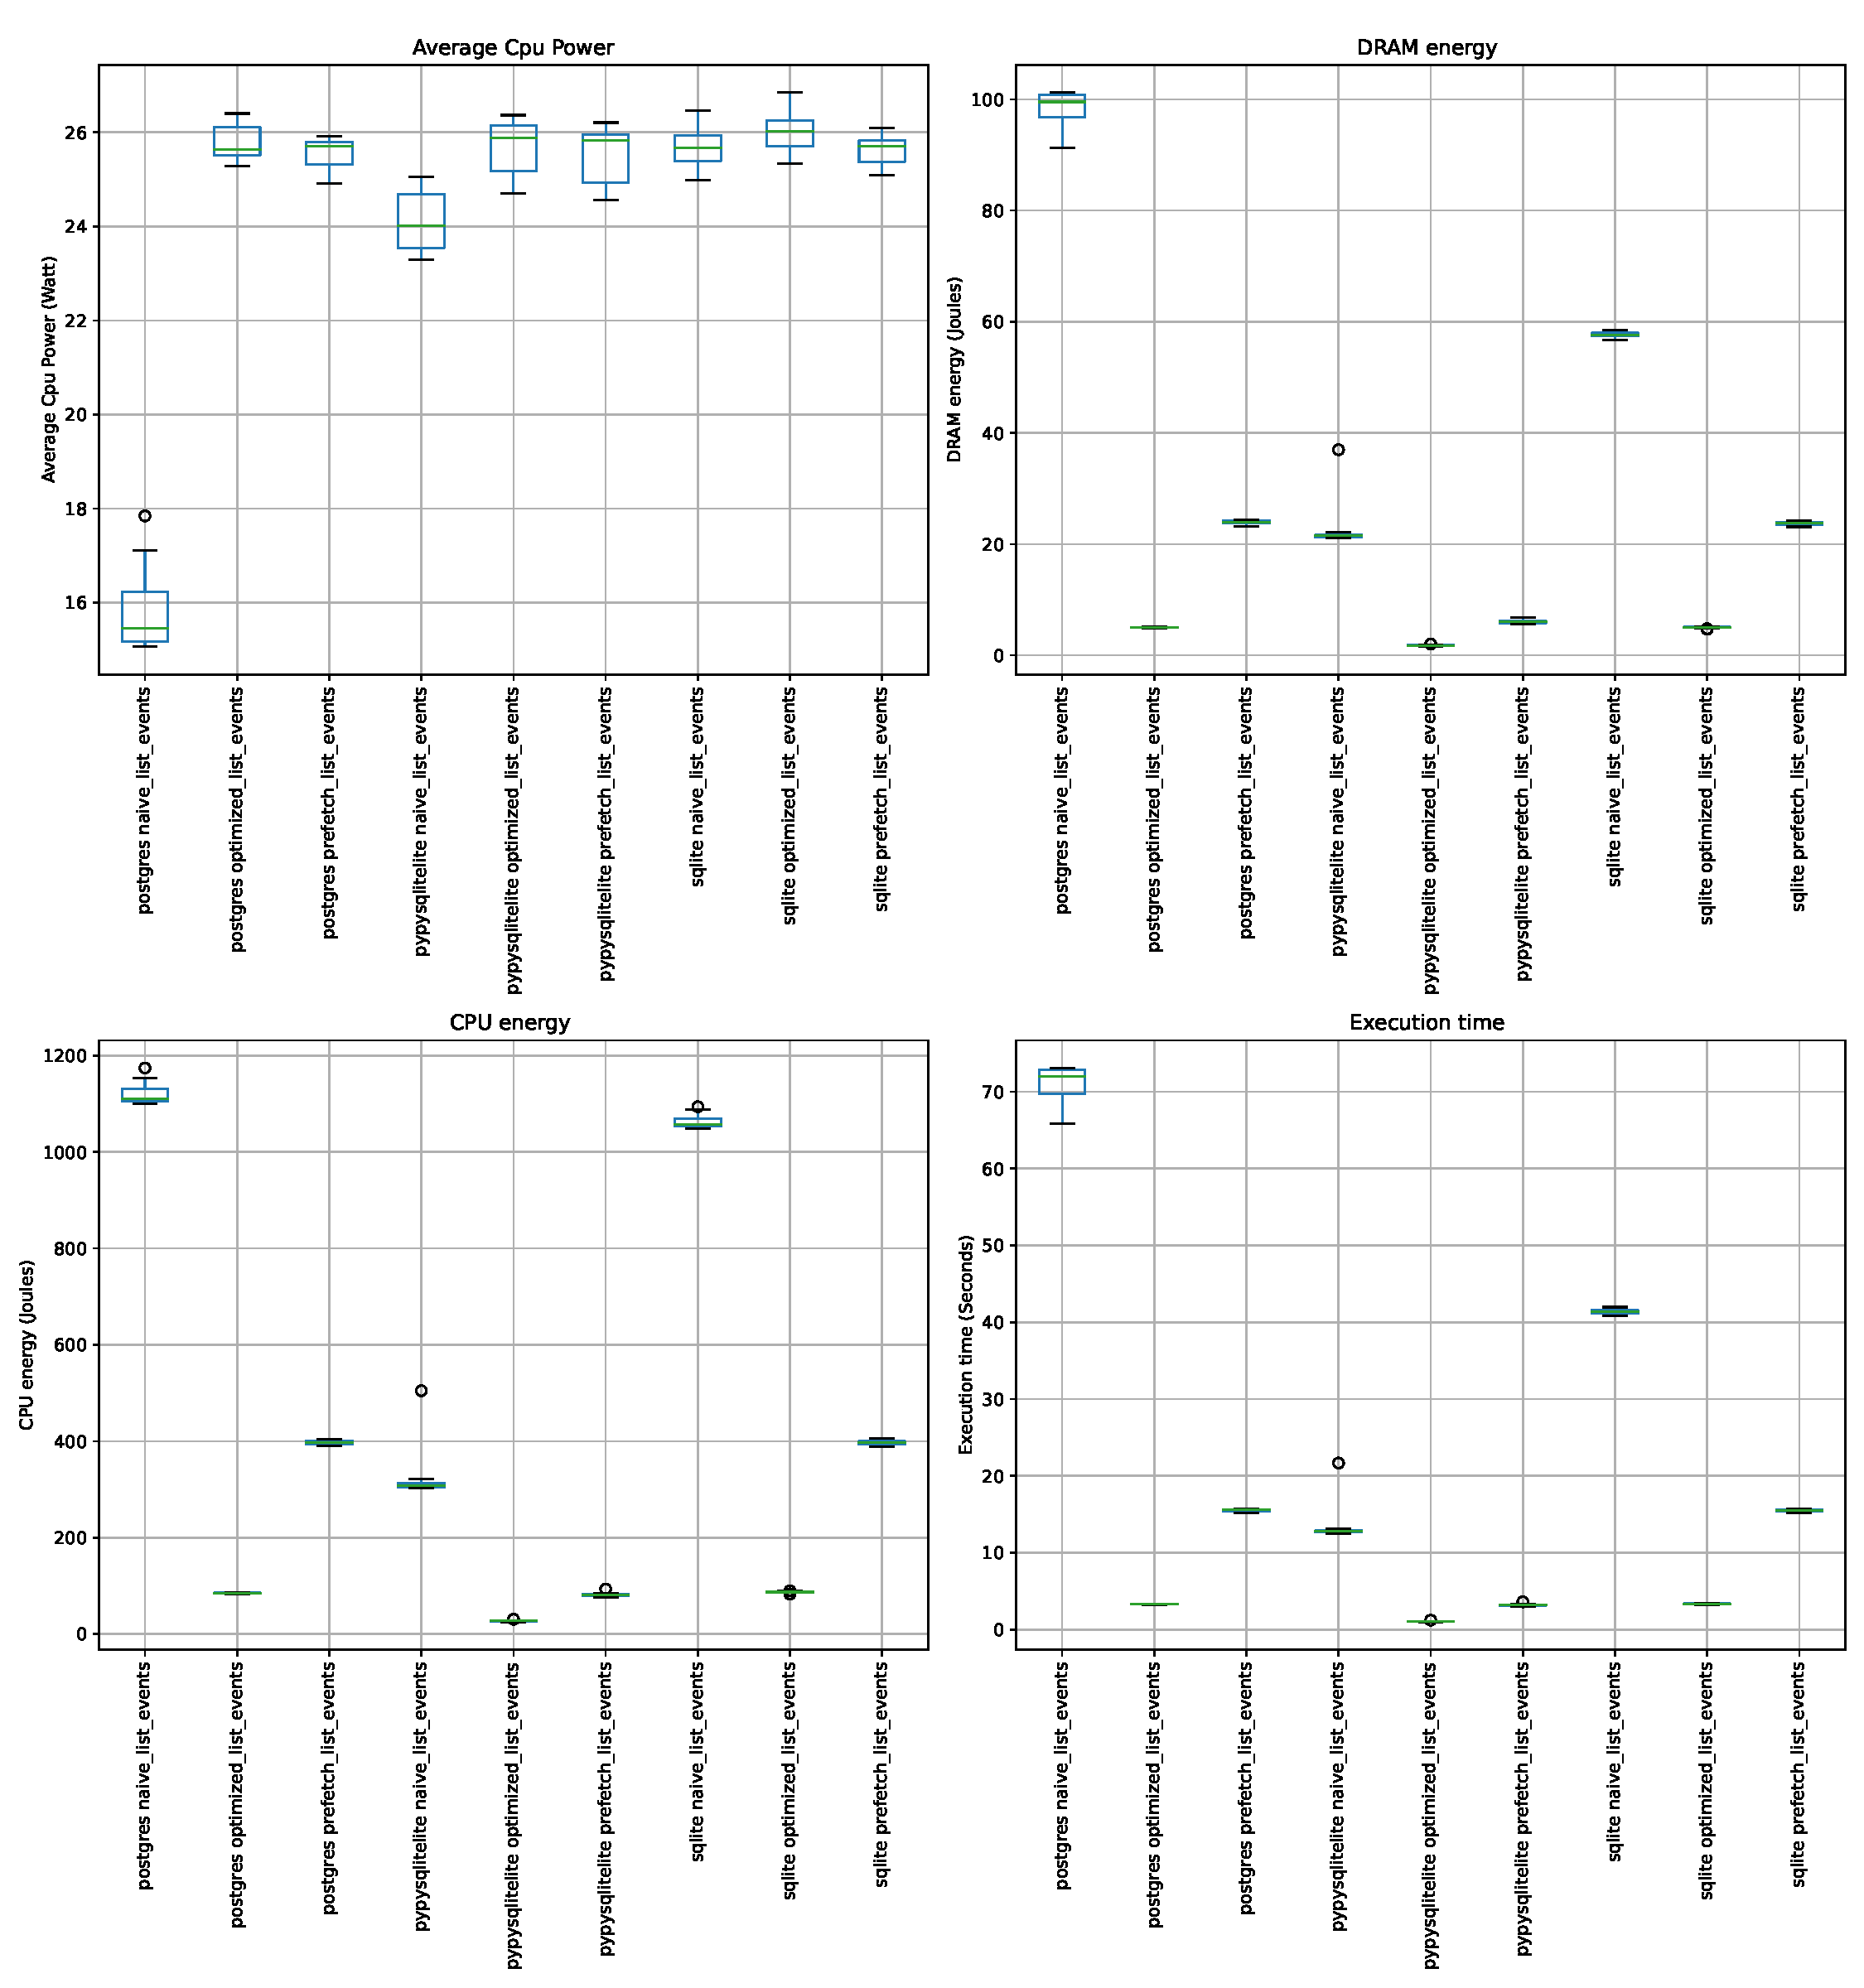
\includegraphics[width=\linewidth]{imgs/django}
    \caption{energy behaviour based on multiprocessing}
    \label{fig:django}
\end{figure}


%%%%% have to rephrase this 

As one can see in figure~\ref{fig:django}, different choices of requesting the data have a huge impact on the energy consumption. as the naive version can consume up to 10x more energy than the optimized one.
In the other hand the choice of the data base didnt have huge impact on the total energy despite their different behaviour regarding the execution time and the average power.
This can be useful to help develeppers make a choice regarding which data base they can use based on the number of the expected requests and the expectation of the performance.

Another interesting observation is the impact of the interpreter, as figure~\ref{fig:django} highligh. the use of Pypy interpter instead of the default one helped reducing the amount of the energy consumption even when we are dealing with the naive version.

Figure \ref{fig:python_multiprocessing} shows the behaviour of python programs when we try to introduce the parallelism.
As we know python is a single threaded program thx to ghe GLS ( global lock system ) howerver due to the increase of the number of cores /threads per cpu it many libraries stared to take advanteage of this feature so most of them they will try to simulate the multithreading by using multiple instances pf the processor % TO VERIFY 

\begin{figure}[hbt]
    \centering
    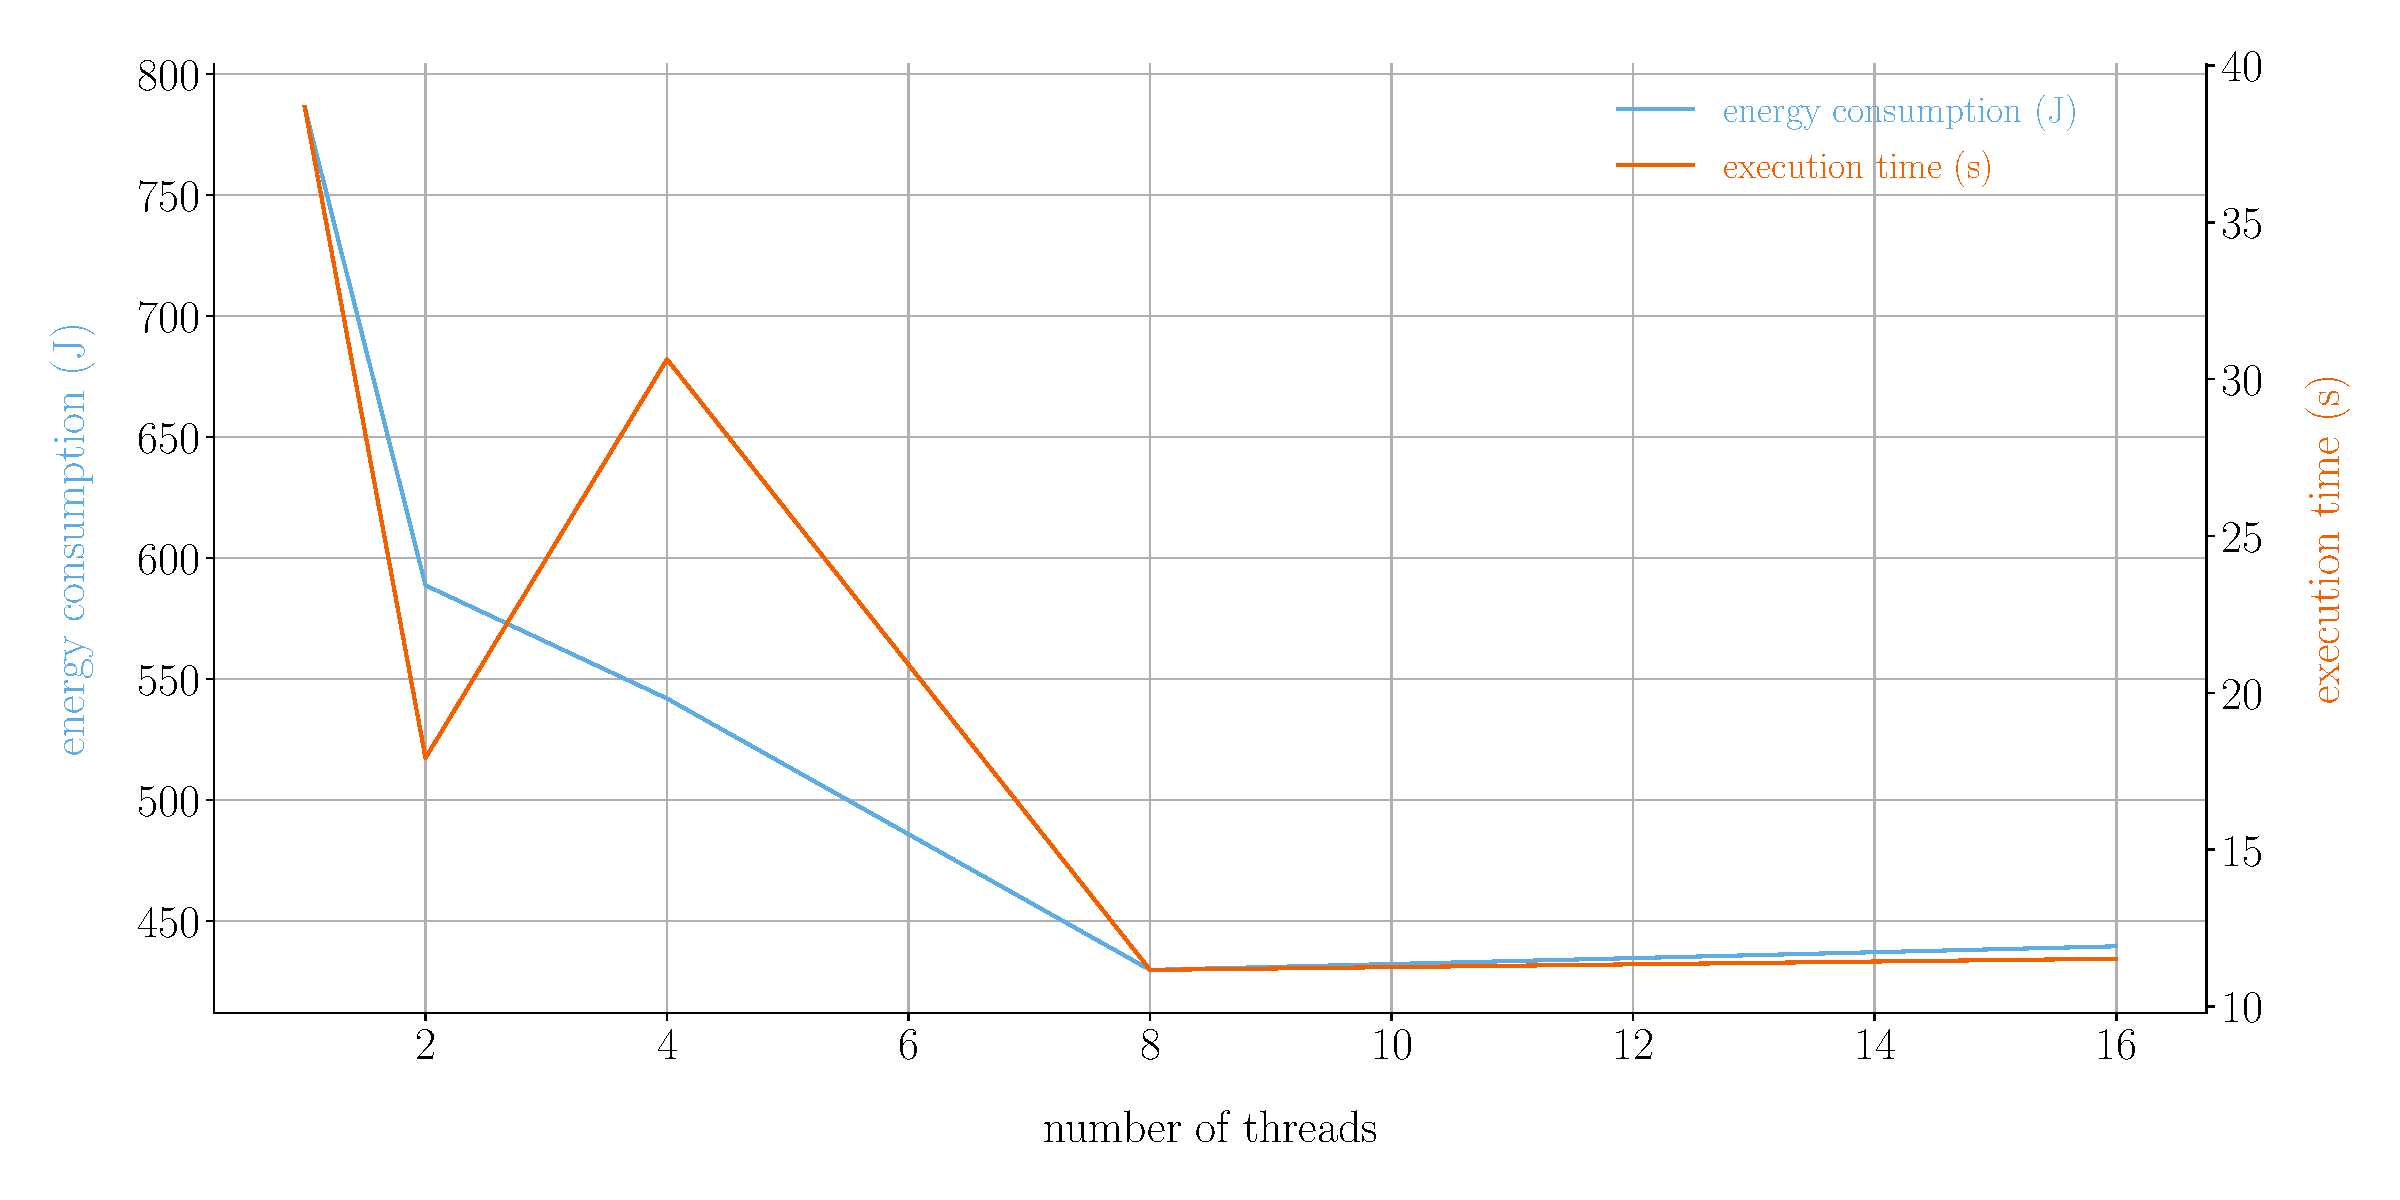
\includegraphics[width=\linewidth]{imgs/multiprocessing_energyvstime}
    \caption{energy behaviour based on multiprocessing}
    \label{fig:python_multiprocessing}
\end{figure}

as we can see in the graph the energy consumption is correlate with the number of threads until we arrive to the limit of the cores and then we lose the adventage of the multiprocessing , well in that case we pass from parallelism to concurency. where different sub process have to compete for the CPU Ressources.
Another finding is when we hit the number of physical cores. there was an increase of execution time but still reduced energy, the reason behind this is the scheduler of the operating system. basicaly he favorits the hyper threads than the physical core wich will lead to some context switches which cause the slow behaviour, howerver in the other hand the other two physical cores are not consuming energy, neither their hyper threads which explains the gain of the eneryg consumption in this case.
in the Chapter %% reference the work of intern from lyon  
we discuss a deeper this behaviour of the scheduler and in that case we confirm that it is not related to python but it is more generic behaviour %% maybe even this graph should go there 


\subsection{python insights}

The goal of this section is to find some insights where we can optimize the energy consumption without impacting the source code. so we started by extending the work of \citeauthor{hasan_energy_2016} and \citeauthor{oliveira_recommending_nodate} to the python environement.



%%%% concurency 



another field of investigation is the type data and structure conroles. that might impact the energy consumption.
To do so. We iterate over a list using three methodes.
first the classical for ( for i in range (len(n))). howerver as we can see here unlike other porgramming langauges it requires extra operations such as determining the length of the collection , and then using the iterator range. so we tried the more adapted version
( for element in collection). Morever in most programming languages the for loop is translated to a while loop ( transfirmation from D type to B type -- asm -- ), therefore we wanted to compare this with a ( while ) version.
After determining the main ways to iterate over a loop we run the algorithms  collections of different data types to see wether it will impact of the energy consumption of the code, same thing for the size of the collection.

As we can see in figure~\ref{fig:pythonloops} the type of the data hasn't an impact on the energy consumption.In the other hand the way we iterate over the collection has a huge factor. interestely, the for in range loop was by far the optimal one with following by the regural for in collection, and the while part was the least one with an overhead of 400\% compared to the first option.



%%% putting the idea, later i ll reformulate it 
the reason behind a such behaviour is mainly related on how python interpeter is made.
% add refenece https://www.python.org/doc/essays/list2str/ 
%% https://www.pythonpool.com/for-vs-while-loop-python/  
% https://wiki.python.org/moin/TimeComplexity
%% http://python-history.blogspot.com/2010/06/from-list-comprehensions-to-generator.html?m=1
In order to reduce the latency of the python code. most of the buitl-in functions an operations are written in C, same thing goes for the function range, further more the function len has a complexity of O(1) because it is based on the function Py\_SIZE  of C which stores the length in a field for the object.
so basically for the for in range is basically creating a new iterator that has the same length of the first one. and for each iteration we will have to do a second acceess ( l[i]) instead of one one access hence the double time.
for the wile is even slower due to the implicite incrementation of the variable which will cause an extra operation during the loop .
to confirm the hyphothsis. we tried to construct a new list by editing the elements of the previous one. And as predicted , the builtin methodes are the best energy saving, while the customize while loop is the heaviest. an interesting finding is. the impact of annonymous functions ( lambda expressions) on the energy consumption.
the reseason behind this is the fact that python treats those functions as local variables unlike the predifined ones which are global in our case. therefore they are faster and consumes less energy  % same reference https://www.python.org/doc/essays/list2str/ 

\begin{figure}
    \centering
    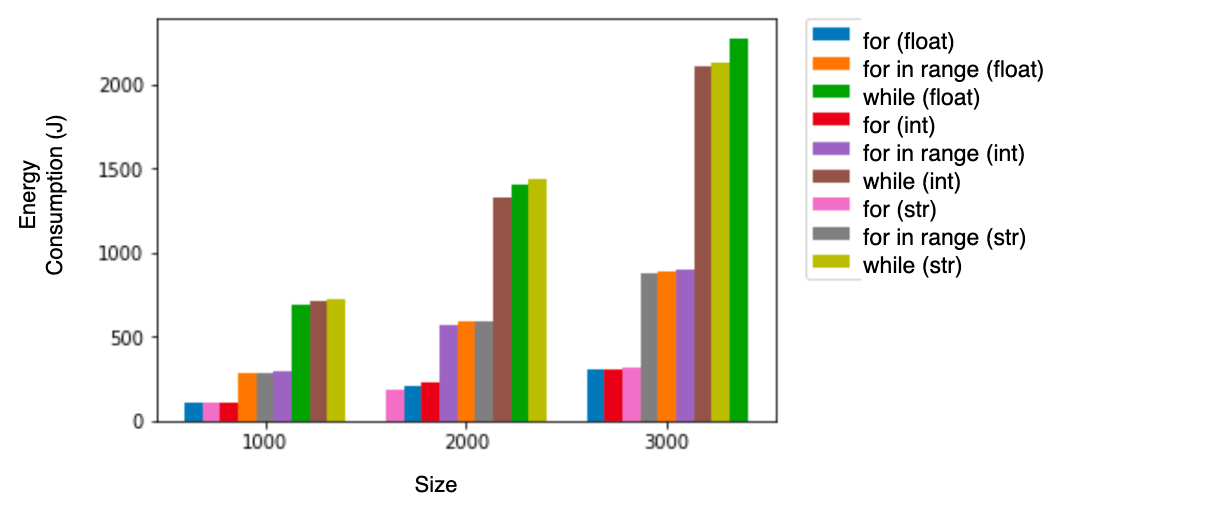
\includegraphics[width=\linewidth]{imgs/python_iterations}
    \caption{energy behaviour of different python loops }
    \label{fig:pythonloops}
\end{figure}


\begin{figure}
    \centering
    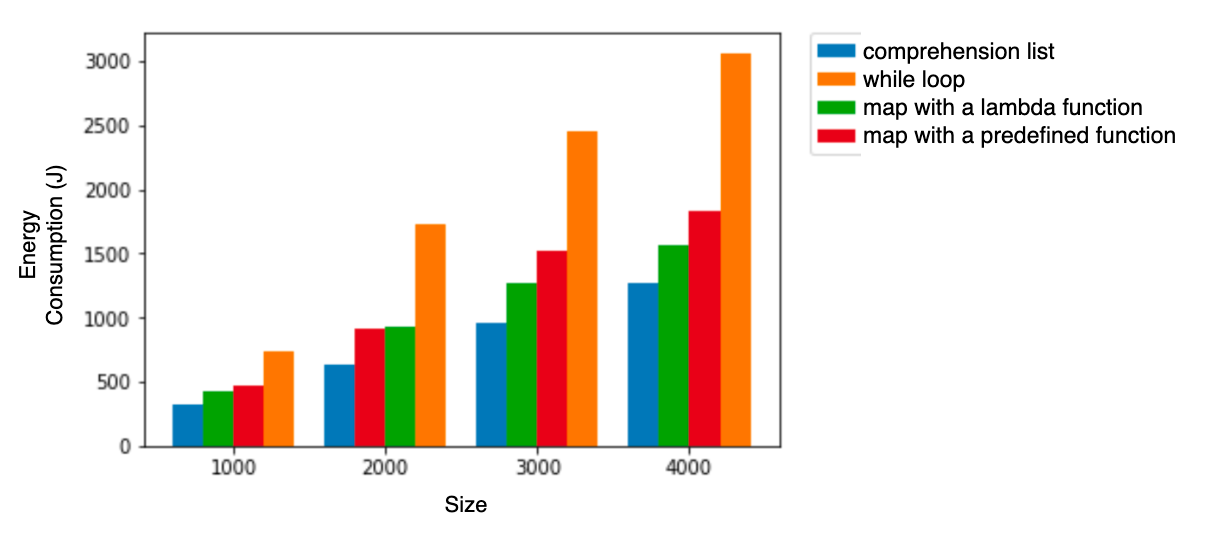
\includegraphics[width=\linewidth]{imgs/python_treatemens}
    \caption{energy behaviour of different methodes to change a list}
    \label{fig:pythontreatement}
\end{figure}

\paragraph{conclusion}
This study has shown us, that the optimial way to reduce the energy consumption of the python code is to follow the guidelines and use the builtin functions, which is kinda happy news for the developers since they don't have to make extra effort to make their code green


\subsection{python and multiprocessing}
Figure \ref{fig:python_multiprocessing} shows the behaviour of python programs when we try to introduce the parallelism.
As we know python is a single threaded program thx to ghe GLS ( global lock system ) howerver due to the increase of the number of cores /threads per cpu it many libraries stared to take advanteage of this feature so most of them they will try to simulate the multithreading by using multiple instances pf the processor % TO VERIFY 

\begin{figure}[hbt]
    \centering
    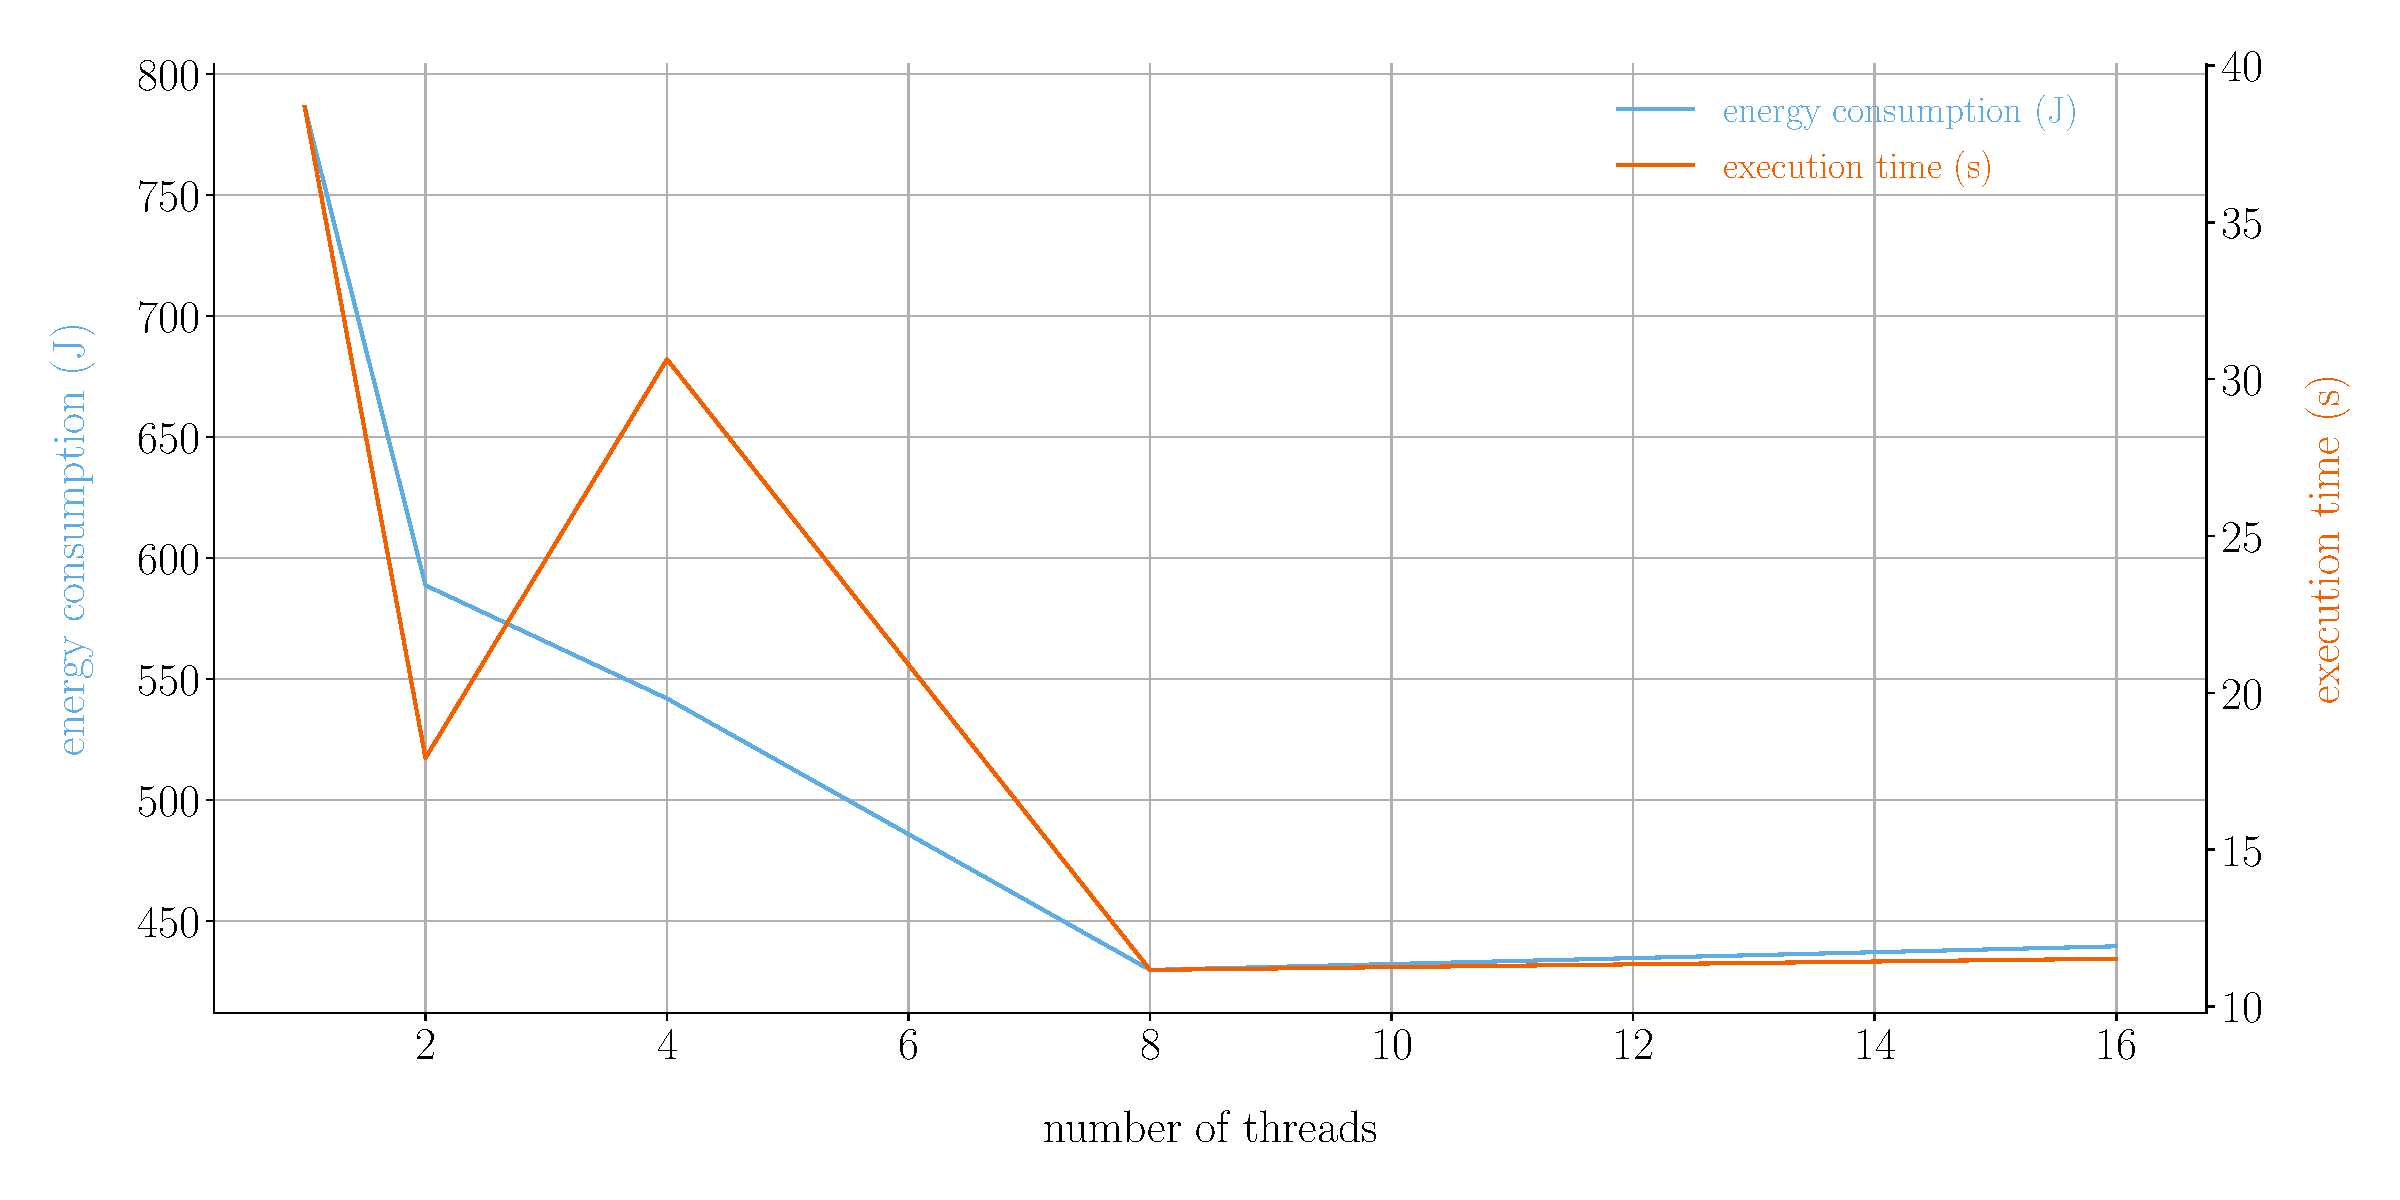
\includegraphics[width=\linewidth]{imgs/multiprocessing_energyvstime}
    \caption{energy behaviour based on multiprocessing}
    \label{fig:python_multiprocessing}
\end{figure}

as we can see in the graph the energy consumption is correlate with the number of threads until we arrive to the limit of the cores and then we lose the adventage of the multiprocessing , well in that case we pass from parallelism to concurency. where different sub process have to compete for the CPU Ressources.
Another finding is when we hit the number of physical cores. there was an increase of execution time but still reduced energy, the reason behind this is the scheduler of the operating system. basicaly he favorits the hyper threads than the physical core wich will lead to some context switches which cause the slow behaviour, howerver in the other hand the other two physical cores are not consuming energy, neither their hyper threads which explains the gain of the eneryg consumption in this case.
in the Chapter %% reference the work of intern from lyon  
we discuss a deeper this behaviour of the scheduler and in that case we confirm that it is not related to python but it is more generic behaviour %% maybe even this graph should go there 

%% todo 
% add performance 
% add dram \ a glimps 

\subsection{Python and machine learning }
\begin{figure}
    \centering
    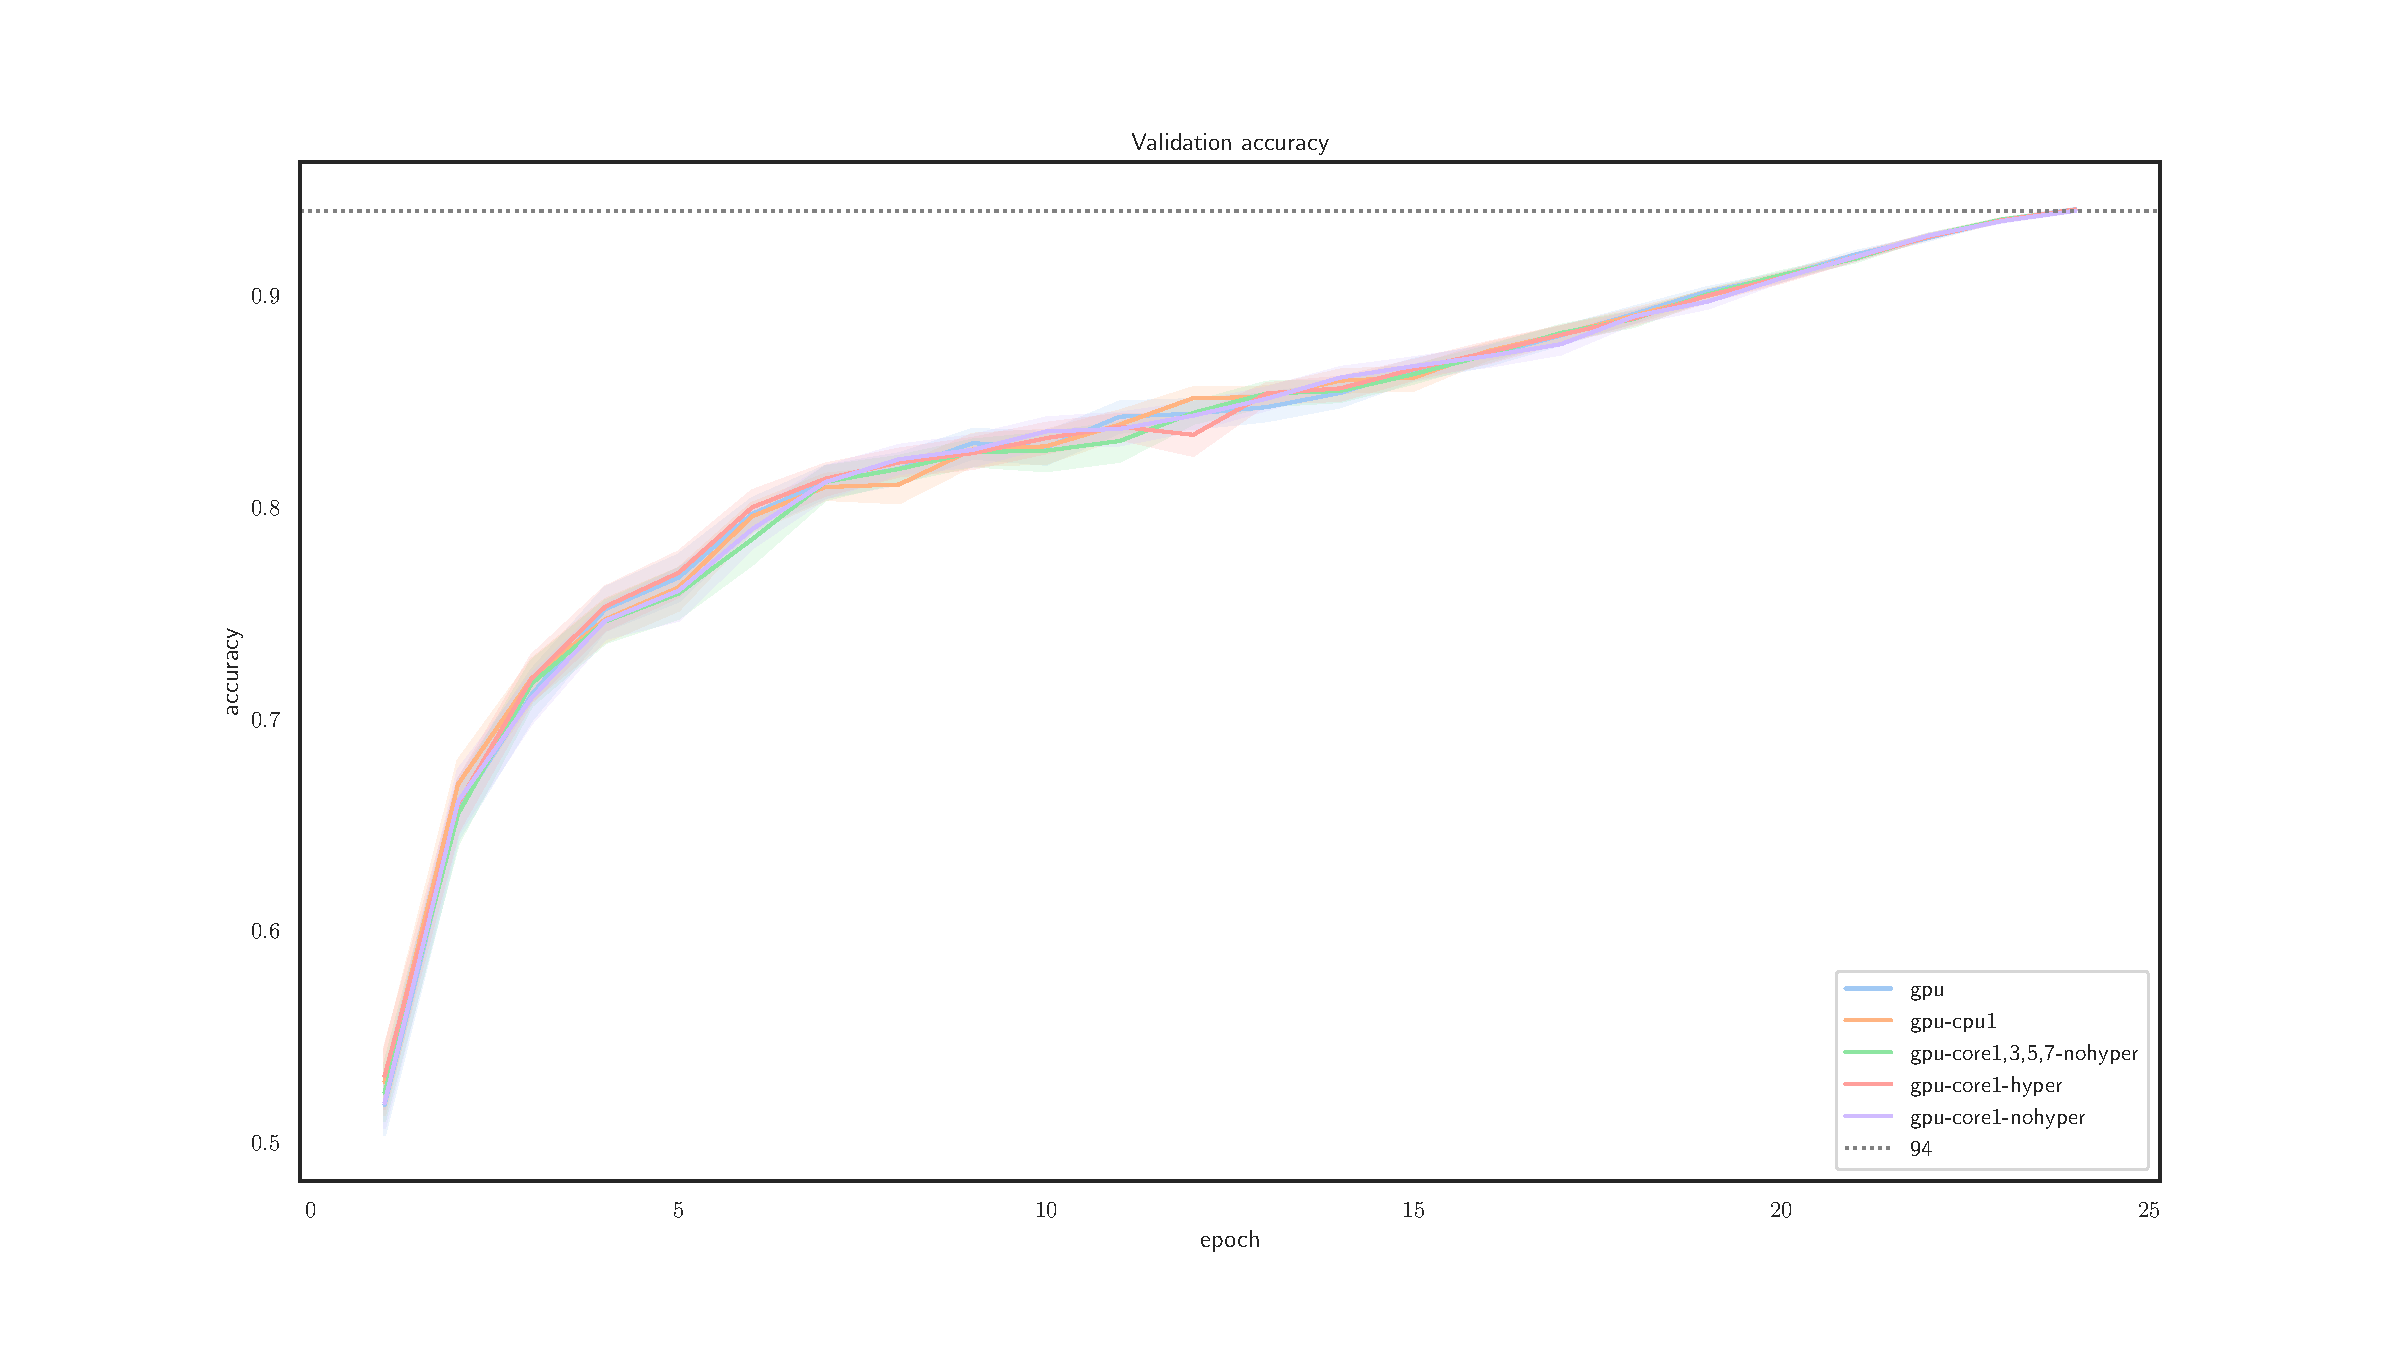
\includegraphics[width=\linewidth]{imgs/accuracy_basedonepoch}
    \caption{accuracy based on epoch  }
    \label{fig:p2}
\end{figure}

\begin{figure}
    \centering
    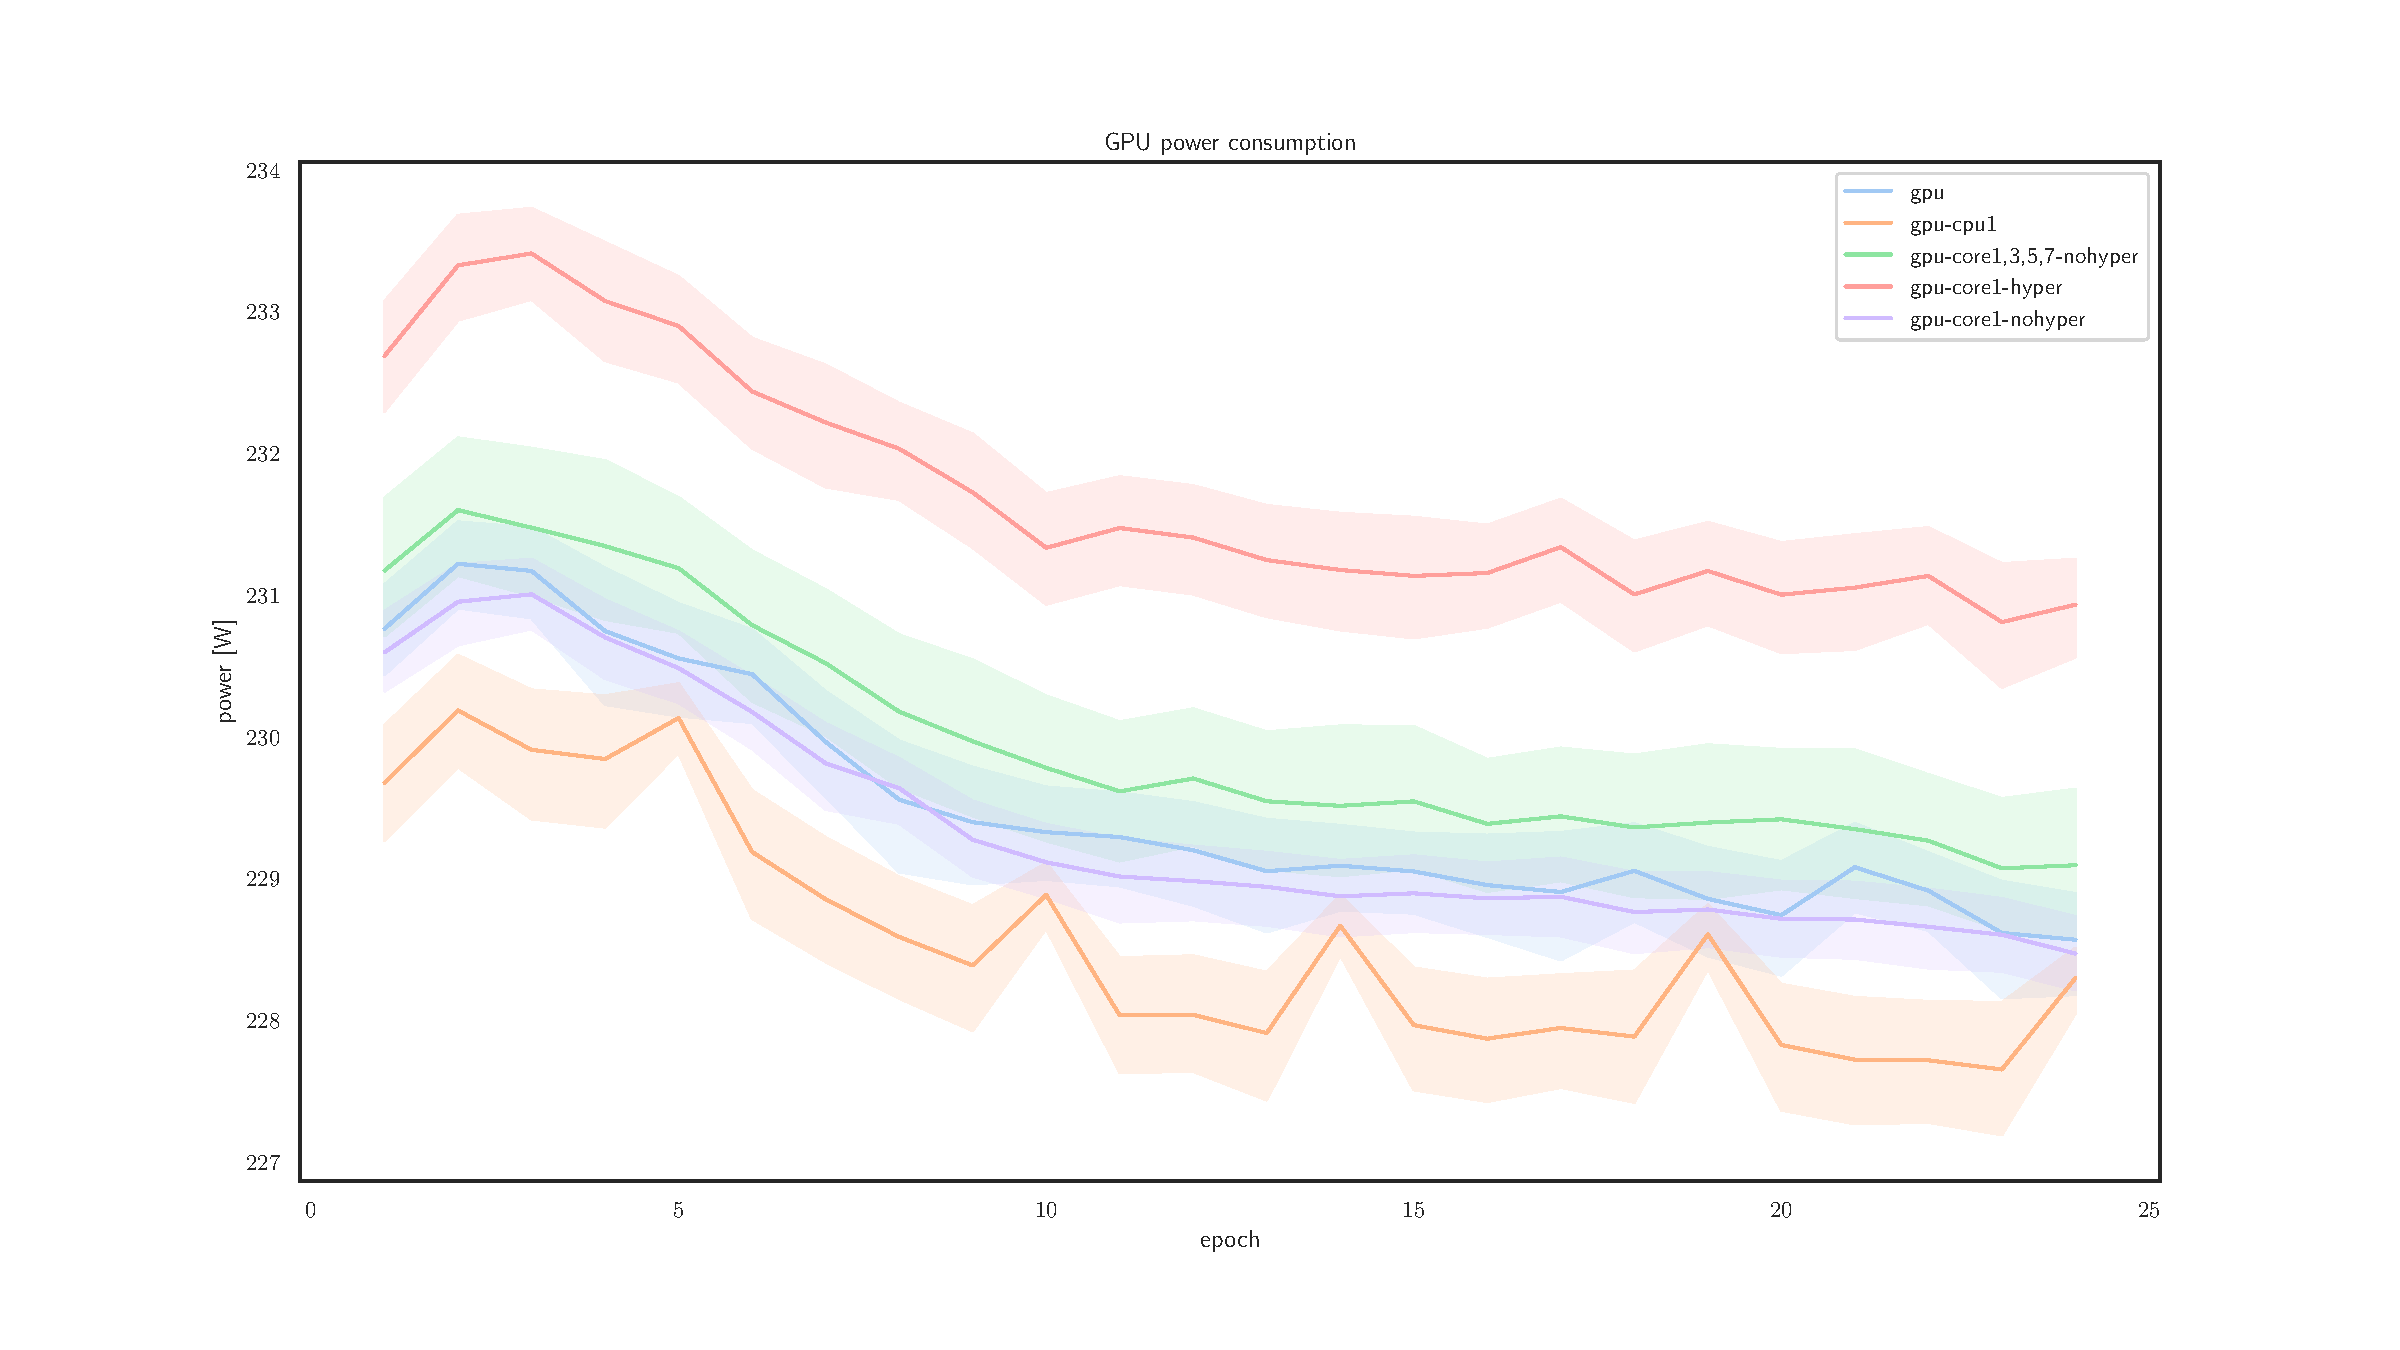
\includegraphics[width=\linewidth]{imgs/power_gpu_baedonepoche}
    \caption{evolution of average gpu power based on epoch  }
    \label{fig:p2}
\end{figure}
\begin{figure}
    \centering
    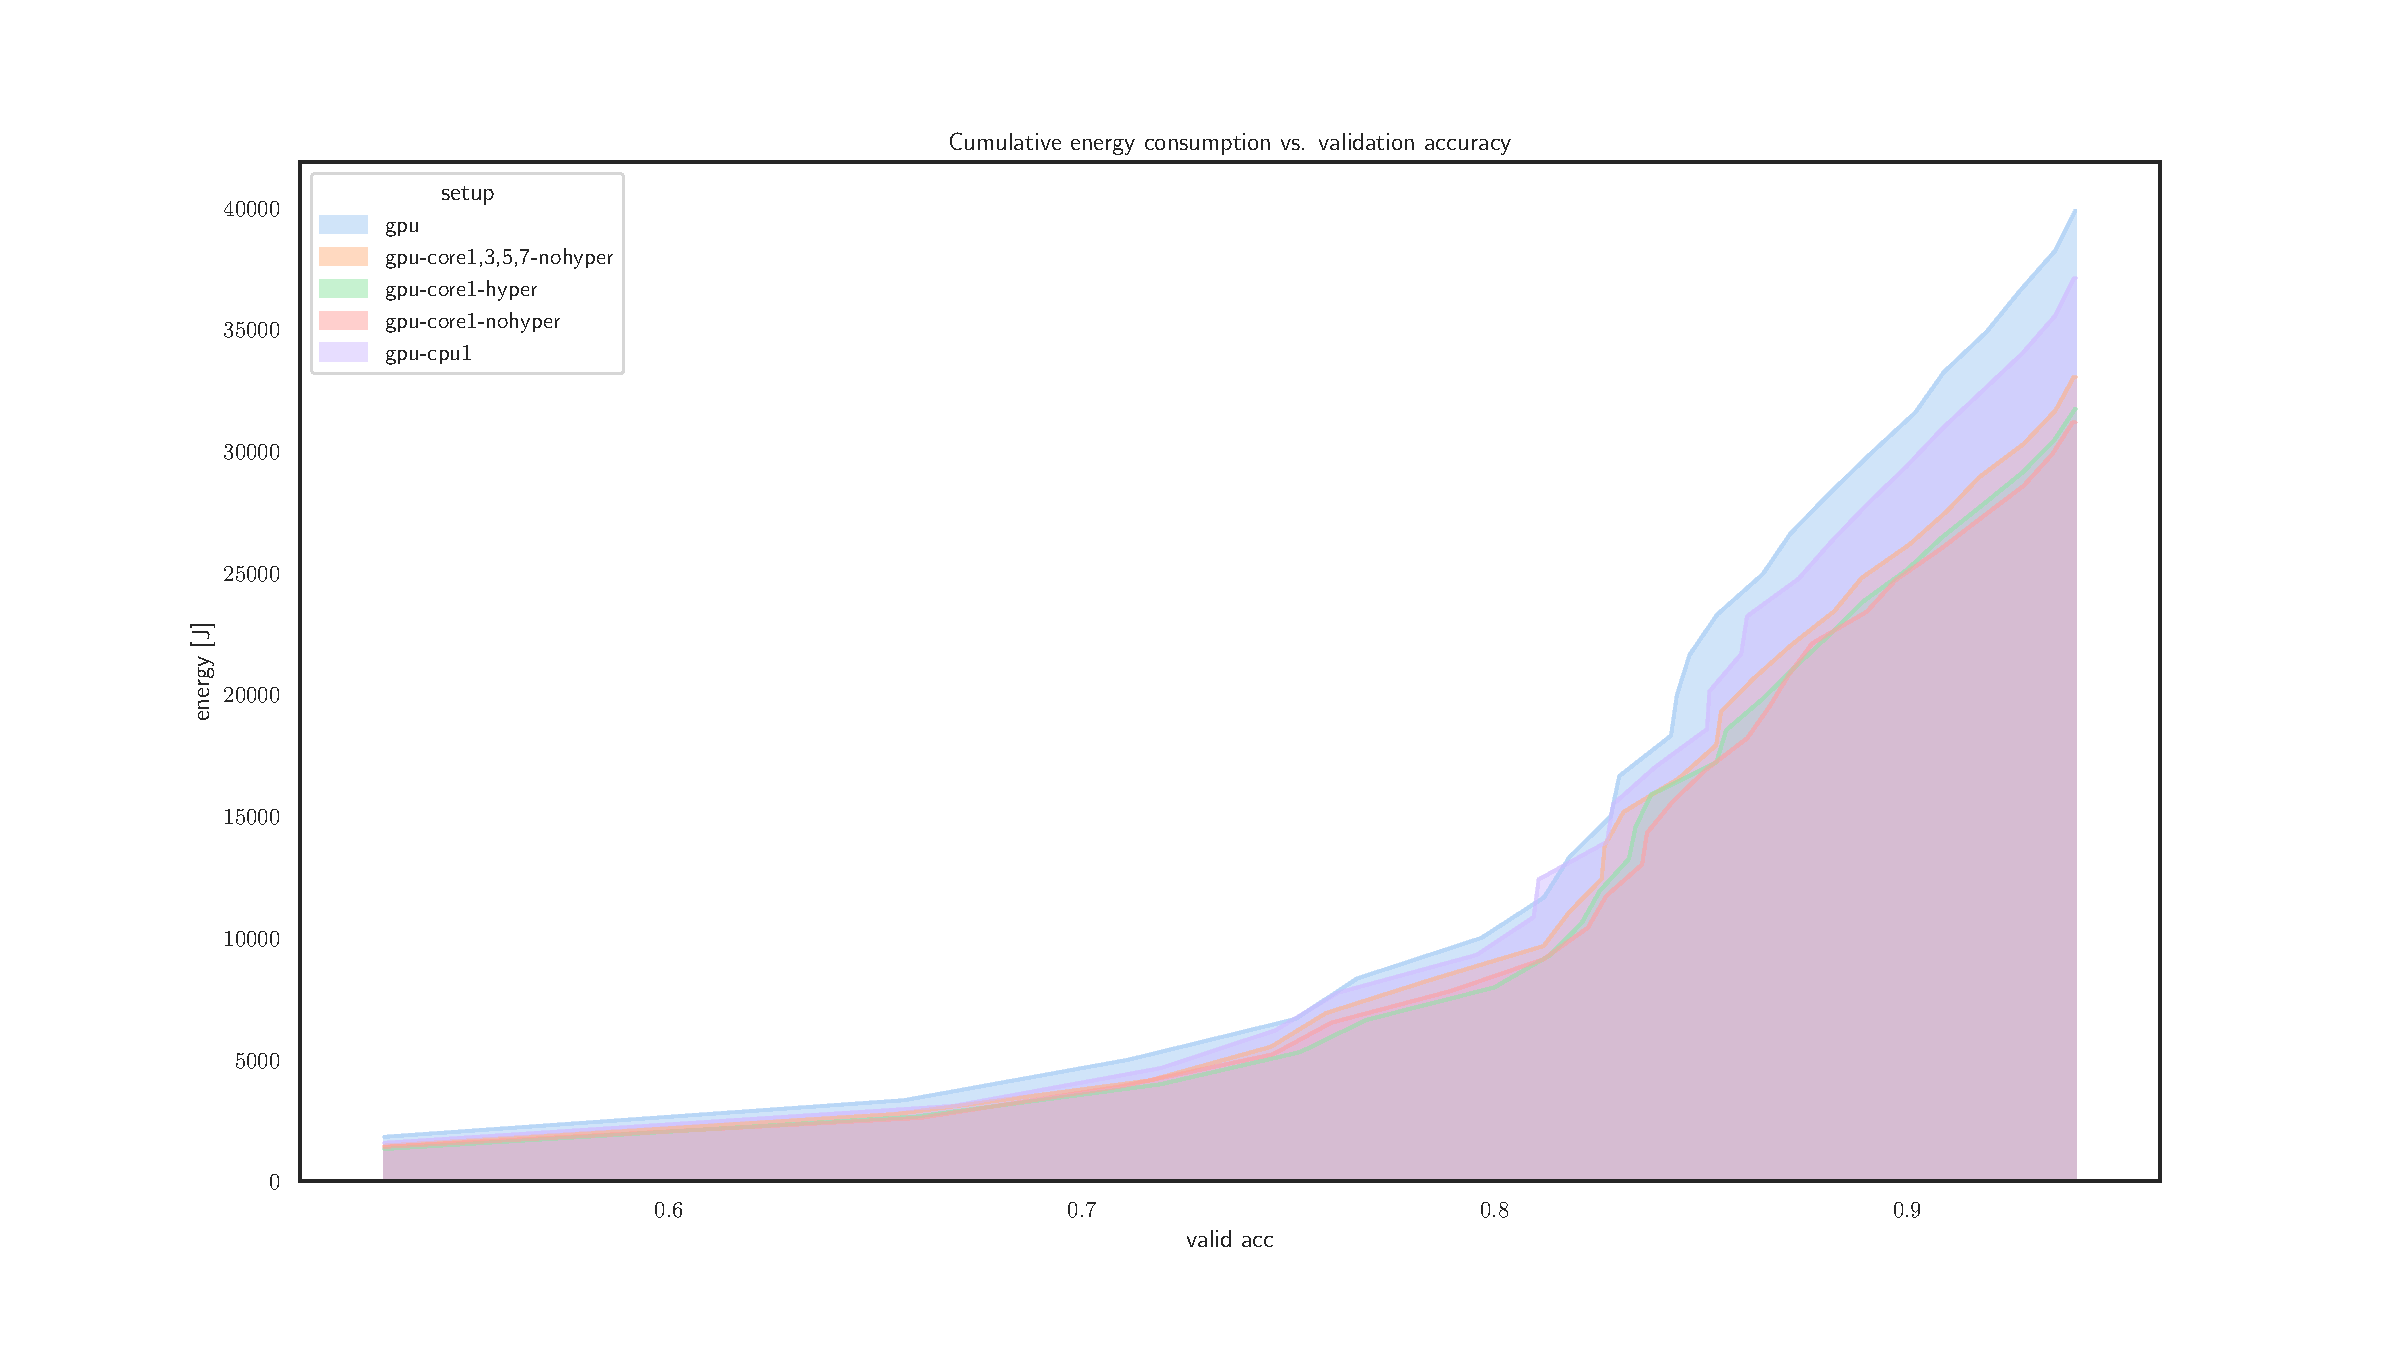
\includegraphics[width=\linewidth]{imgs/cumulative_energy_fast10}
    \caption{cumulative energy of fast10 benchmark within different configurations }
    \label{fig:p2}
\end{figure}



\paragraph{conclusion}
We discovered that when a model's accuracy improves, so does the energy required for a subsequent accuracy gain.
This begs the question of when we should discontinue training.
Is a 10\% increase in accuracy worth it if we have to spend three times the energy?
Even while utilizing a GPU consumes more total power, the training time is significantly reduced.
As a result, the utilization of a GPU is required to lower the energy consumption of the training.
Some experiments revealed unusual behavior that was not studied during this internship.
These could be examined in future studies and perhaps used to achieve more energy savings.
The execution time did not depend on the number of cores employed in several studies.
This parameter had a significant impact on training time in others.
As a result, the best core configuration will be determined by the script.
The next steps in this area could include exploring the reasons for these discrepancies and possibly creating a script that can automatically find the ideal core configuration for a specific script.







\section{Python interpreters}\label{sec:pythoninterpreters}

%%% note : add this to the section of python interpreters 
Due to the lack of of support for most of  non conventional pyton interpeters, our main focus was only on micro benchmarks.
Except pypy most of the python implementations don't support extra python libraries, Despite that most of the cases those extra implementations were made to optimize a specific library such as numba with numpy, or intelpython with machine learning algorthms.

\paragraph{preliminary studies}
For the first studies we used only the official version of python. because the goal was mainly to highlight the impact of the structure of code on the energy consumption.
One main inconvienent of the previous methode to reduce the energy consumption, is the hard work that should be done in order to alter the existing code base in order to redcue the energy consumption. To avoid such hustle we tried to find a non intrusive way to make the python code more ecofriendly without changing its structure. One aspect of python is the fact that it is an interptered language which led many works to create their own implementation of the interpeter to enhance one or many aspect of the python code. in the following section we will discuss the impact of those implementations on the energy consumption of python programs, and in which case, one should use a non conventional interpter to save the energy consumption of their program.

To do so, we gathered a list of interpeters, transpilers and some optimization libraries.

the following list, presents the most famous ones .
% We should explain the methodology we used to select these

\begin{enumerate}
    \item \textbf{CPython}:\footnote{\url{https://www.python.org/}} a Python interpreter written in C programming language. It is the reference interpreter of Python. CPython compiles the source code into a bytecode and then interprets it. The CPython project still supports both versions of Python 2 and 3;
    \item \textbf{PyPy}:\footnote{\url{http://pypy.org}} An alternative implementation of the Python interpreter. It is written using \emph{RPython} in order to use the JIT. It compiles the most used portions of the Python code into a binary code for better performance. To benefit from these optimizations, the program has to be executed for at least for few seconds so the JIT has enough time to warm up, the JIT optimization will be applied only the code written by the programmer and not external libraries;
    \item \textbf{Cython}:\footnote{\url{https://github.com/cython/cython}} a static compiler for Python. It translates the Python code into a C code, and then compiles it using a C compiler. It also support(s) an extended version of the Python language that allows programmers to call \emph{C functions}, declare \emph{C types} and use static types which will help the translation of Python objects into native types, such as integers, float, which often means a better performances, since native C libraries are almost all the time faster than the python written once~\cite{pereira_energy_2017}.
    \item \textbf{Intel\,Python}:\footnote{\url{https://software.intel.com/en-us/distribution-for-python}} A customized interpreter developed by Intel in order to enhance performances of Python programs. It is dedicated to data sciences, high-Performance computing. It uses some Intel kernel libraries, such as Math Kernel Library (Intel MKL\footnote{\url{https://software.intel.com/en-us/mkl}}) and data analytics acceleration library (Intel DAAL\footnote{\url{https://software.intel.com/en-us/intel-daal}}). It supports both versions of Python;
    \item \textbf{Active\,Python}:\footnote{\url{https://www.activestate.com/products/activepython/}} developed by the Activestates company, it provides a standardized Python distribution to ensure license compliance, security, compatibility and performance. Therefore, ActivePython has its own built-in packages (more than 300 packages) and supports both versions of Python;
    \item \textbf{IronPython}:\footnote{\url{https://ironpython.net}} A .Net-based Python interpretation platform written in C\# in order to be used over the .Net vm or mono, it benefits from all the optimizations of .Net virtual machine, such as the JIT and garbage collector mechanisms.
    \item \textbf{GraalPython}:\footnote{\url{https://github.com/graalvm/graalpython/}} A Python interpreter that is based on GraalVM \footnote{\url{https://www.graalvm.org/docs/why-graal/}} (a universal virtual machine developed by oracle for running applications written in different programming languages). For the time being, it only supports Python~3 and it is still in the experimental stage;
    \item \textbf{Jython}:\footnote{\url{https://jython.github.io}} Implementation of Python programming language written in Java for the \emph{Java virtual machine} (JVM). Similar to IronPython and GraalPython, it leverages the optimization mechanisms provided by the JVM to enhance the Python programs;
    \item \textbf{MicroPython}:\footnote{\url{http://micropython.org}} a lightweight Python version dedicated to embedded systems and micro-controllers;
    \item \textbf{Nuitka}:\footnote{\url{http://nuitka.net/pages/overview.html}} a Python compiler written in Python that generates a binary executable from Python code. It translates the Python code into a C program that is then compiled into a binary executable;
    \item \textbf{Numba}:\footnote{\url{https://numba.pydata.org}} a library that includes JIT compiler in order to enhance the performances of Python functions using the industry-standard LLVM compiler library;
    \item \textbf{Shedskin}:\footnote{\url{https://github.com/shedskin/shedskin}} a static transpiler that translates implicitly statically typed python into C++ code.
    \item \textbf{Hope}~\cite{akeret_hope_2015}: a Python library that aims to introduce JIT compiler into the Python code;
    \item \textbf{Parakeet}~\cite{DBLP:conf/hotpar/RubinsteynHWS12}: a runtime accelerator for an array-oriented subset of Python;
    \item \textbf{Stackless\,Python}:\footnote{\url{https://github.com/stackless-dev/stackless/wiki}} an interpreter that focus on enhancing multi-threading programming.
    \item \textbf{Pyjion}:\footnote{\url{https://github.com/microsoft/pyjion}} JIT API for CPython, same purpose as Parakeet and Hope.
    \item \textbf{Pyston}:\footnote{\url{https://blog.pyston.org}} performance-oriented Python implementation built using LLVM and modern JIT techniques. the project is funded by dropbox;
    \item \textbf{Grumpy}:\footnote{\url{https://github.com/google/grumpy}} a source-to-source transpiler that translates the Python code into a Go code that will be compiled to a binary executable. It also offers an interpreter called \emph{grumprun} which can directly execute the Python code. Unfortunately, we cannot use it because the project is already outdated (last commit is in 2017) and it has a lot of limitation in term of supporting the Python language, such as some built-in functions and standard libraries;
    \item \textbf{Psyco}:\footnote{\url{http://psyco.sourceforge.net}} a JIT compiler for Python;
    \item \textbf{Unladen\,Swallow}:\footnote{\url{https://unladen-swallow.readthedocs.io/en/latest/}} an attempt to (use) LLVM  as  JIT compiler for CPython.
\end{enumerate}


\subsection{Runtime Classification}
Before futher proceeding with the list of candidate runtimes for Python applications, we propose a classification according to several criterions:
\begin{description}
    \item[\bf Type] refers to the category of runtime infrastructure that supports the execution of a Python application. In particular, we consider 3 types of environments: \emph{Interpreter}, \emph{Compiler} and \emph{Library}. \emph{Interpreter} refers to the class of environment that does not require any preprocessing of Python source code. \emph{Compiler} introduces a compilation phase prior to the execution of the application. Finally, \emph{Library} induces some modification of the source code.
    \item[\bf Runtime] refers to the technology supporting the execution of a Python application. This technology can refer to the programming language used to program the interpreter, the target language for a compiler or a library.
    \item[\bf JIT optimisation] refers to the support of \emph{just-in-time} compilation in the runtime infrastructure supporting the execution of the application.
    \item[\bf GC optimisation] refers to the support of \emph{garbage collection} in the runtime infrastructure supporting the execution of the application.
    \item[\bf Python version(s)] refers to the list of Python source code versions supported by the runtime environment.
\end{description}

We should explain the classification of these runtimes

\begin{table}
    \caption{Classification of Python implementations}
    \label{fig:python-classes}
    \center
    \begin{tabular}{|l|c|c|c|c|c|c|}
        \hline
        \multirow{2}{*}{\bf Name} & \multirow{2}{*}{\bf Type} & \multirow{2}{*}{\bf Runtime} & \multicolumn{2}{c|}{\bf Optimisations} & \multicolumn{2}{c|}{\bf Python}                     \\
        % \cline{1-5} 
                                  &                           &                              & {\bf JIT}                              & {\bf GC}                        & {\bf 2} & {\bf 3} \\
        \hline
        \hline
        CPython                   & Interpreter               & C                            & \no                                    & \no                             & \yes    & \yes    \\
        \hline
        Intel\,Python             & Interpreter               & C                            & \no                                    & \no                             & \yes    & \yes    \\
        \hline
        ActivePython              & Interpreter               & C                            & \no                                    & \yes                            & \yes    & \yes    \\
        \hline
        PyPy                      & Interpreter               & Python                       & \yes                                   & \yes                            & \yes    & \yes    \\
        \hline
        IronPython                & Interpreter               & .Net                         & \yes                                   & \yes                            & \yes    & \yes    \\
        \hline
        GraalPython               & Interpreter               & GraalVM                      & \yes                                   & \yes                            & \no     & \yes    \\
        \hline
        Jython                    & Interpreter               & Java                         & \yes                                   & \yes                            & \yes    & \no     \\
        \hline
        Stackless\,Python         & Interpreter               & python                       & \no                                    & \no                             & \yes    & \no     \\
        \hline
        MicroPython               & interpreter               & c                            & \no                                    & \no                             & \no     & \yes    \\
        \hline
        Pyston                    & interpreter               & LLVM                         & \yes                                   & \no                             & \yes    & \no     \\
        \hline
        Unladen\,Swallow          & Interpreter               & LLVM                         & \yes                                   & \no                             & \yes    & \no     \\
        \hline
        Cython                    & Compiler                  & C                            & \no                                    & \no                             & \yes    & \yes    \\
        \hline
        Nuitka                    & Compiler                  & C                            & \no                                    & \no                             & \yes    & \yes    \\
        \hline
        Shedskin                  & Compiler                  & C++                          & \no                                    & \no                             & \yes    & \yes    \\
        \hline
        Grumpy                    & Compiler                  & Go                           & \no                                    & \no                             & \yes    & \yes    \\
        \hline
        Numba                     & Library                   & C                            & \yes                                   & \no                             & \yes    & \yes    \\
        \hline
        Hope                      & Library                   & python                       & \yes                                   & \no                             & \yes    & \yes    \\
        \hline
        Psyco                     & Library                   & python                       & \yes                                   & \no                             & \yes    & \yes    \\
        \hline
        Pyjion                    & Library                   & .NET Core                    & \yes                                   & \no                             & \yes    & \yes    \\
        \hline
        Parakeet                  & library                   & C                            & -                                      & \no                             & \yes    & \no     \\
        \hline
    \end{tabular}
\end{table}



\begin{table}[hbt]
    \caption{Classification of Python implementations}
    \label{fig:pythonimplementations}
    \center
    \begin{tabular}{|l|c|c|c|}
        \hline
        Version  & Interpreter     & Transpiler/Compiler & Jit library \\
        \hline
        \hline
        Python~2 & Cpython2        & Cython2             & Numba 2     \\
        % \cline{2-4} 
                 & Pypy2           & Shesdskin           & Hope        \\
        % \cline{2-4} 
                 & Pytson          & Grumpy              & Parakeet    \\
                 & Ironpython      &                     & Psyco       \\
                 & Jython          &                     & Pyjion      \\
        % &  &  &  \\
                 & Micropython     &                     &             \\
                 & Pysec           &                     &             \\
                 & StacklessPython &                     &             \\
        % \cline{2-4} 
        \hline
        Python~3 & Cpython3        & Nuitka              & Numba3      \\
                 & Pypy3           &                     &             \\
                 & GraalPython     &                     &             \\
        \hline
    \end{tabular}
\end{table}

There are other implementations that we didn't considerate because either the project aborted many years ago or it has a very limited support for python features.
After the collection of those implementation we filtered them. in order to keep only the versions that are still maintained and support most of python features.
and we classified them into 3 categories depending of their integration with the python code.  In the \ref{fig:pythonimplementations} we describe the implementations that we kept and the version of each implementation and its category.


\begin{figure}
    \centering
    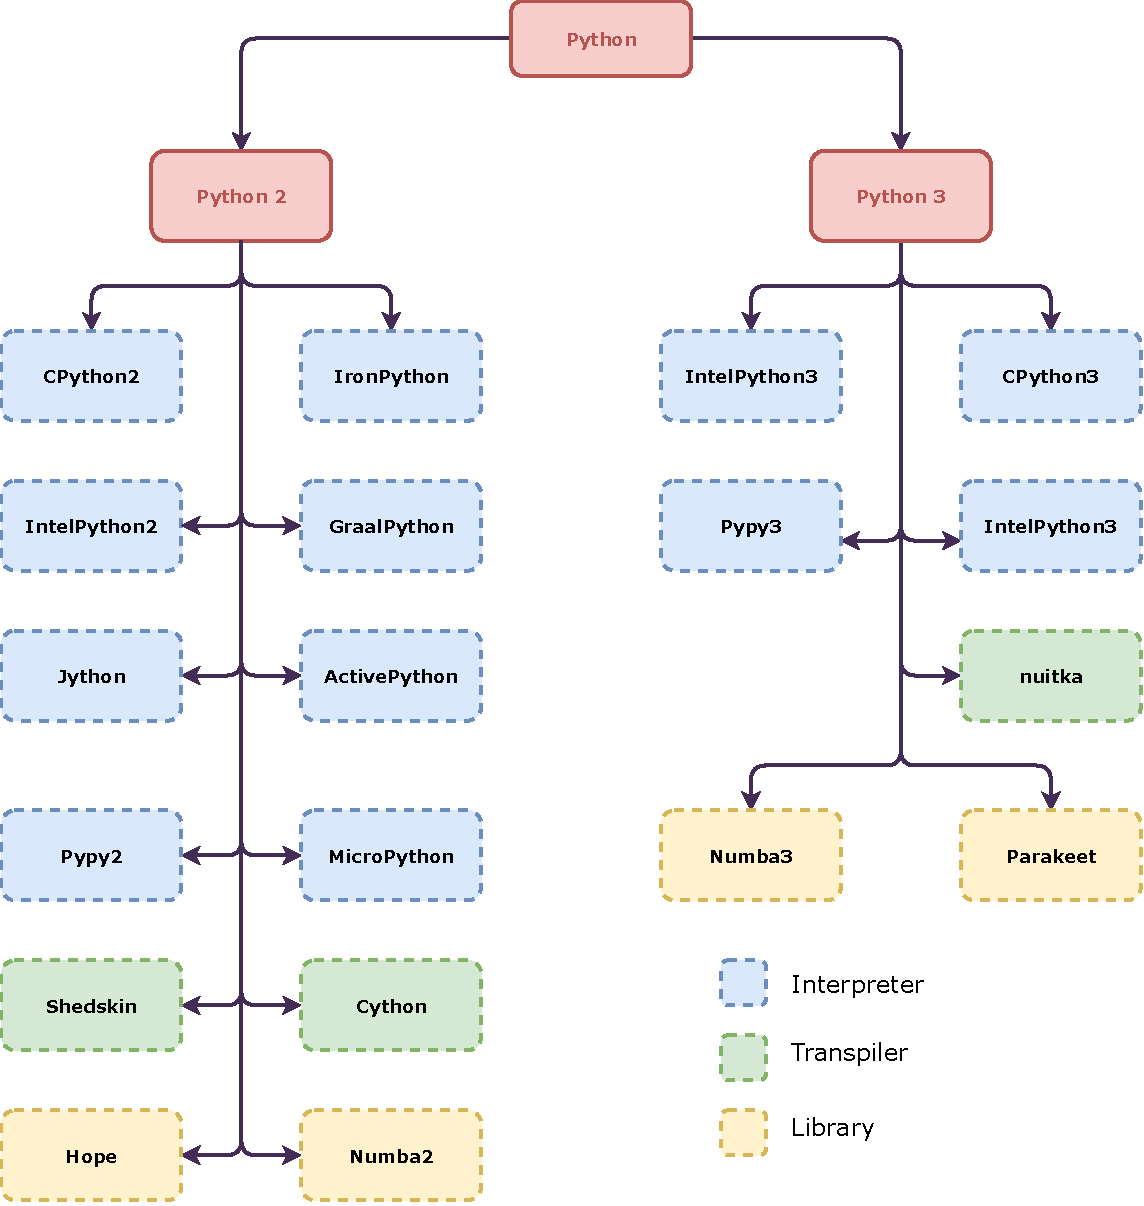
\includegraphics[width=\linewidth]{imgs/python-implementations-tree}
    \caption{Python interpeters}
    \label{fig:interpreters}
\end{figure}



\section{experimetal protocole}

As we have discussed in the previous chapter \ref{chapter:benchmarking}. instead of running the tests, the idea was to design a system that allows practiouners to reproduce and extends our tests. and then we use the same system to run answer some of researchs question.
%%%% probably ill resue the same things from other chapters 
\subsection{measurement context}
\paragraph{Hardware settings}

all our tests have been executed in a Dell PowerEdge C6420 server machine. A summary of its hardware is listed in table \ref{fig:dahuconfig}. The machine is equiped with a minimal version of Debian\,9 (4.9.0 kernel version) where we install Docker (version 18.09.5).



\begin{table}[hbt]
    \begin{tabular}{ll}
        \hline
        CPU     & Intel Xeon Gold 6130 (Skylake, 2.10GHz, 2 CPUs/node, 16 cores/CPU)                                                     \\
        Memory  & 192 GiB                                                                                                                \\
        Storage & 240 GB SSD SATA Samsung MZ7KM240HMHQ0D3                                                                                \\
                & 480 GB SSD SATA Samsung MZ7KM480HMHQ0D3                                                                                \\
                & 4.0 TB HDD SATA Seagate                                                                                                \\
        Network & eth0/enp24s0f0, Ethernet, configured rate: 10 Gbps, model: Intel Ethernet Controller X710 for 10GbE SFP+, driver: i40e \\
                & ib0, Omni-Path, configured rate: 100 Gbps, model: Intel Omni-Path HFI Silicon 100 Series [discrete], driver: hfi1      \\
        \hline
    \end{tabular}
    \caption{Testing Machine Configuration }
    \label{fig:dahuconfig}
\end{table}

\begin{figure}[hbt]
    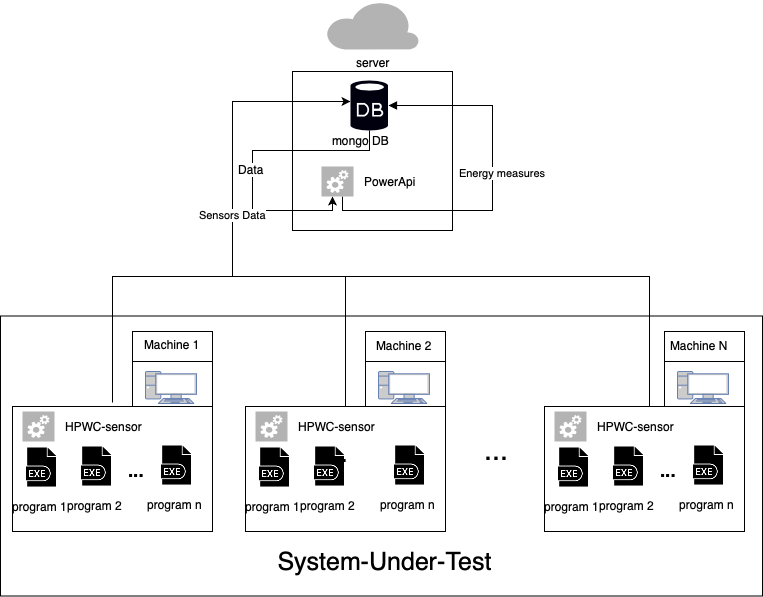
\includegraphics[width=\linewidth]{imgs/SmartWatts.png}
    \caption{powerapi architecture}
    \label{fig:powerapi}
\end{figure}

\paragraph{software settings}
For the sake of reproducibility, each experiment runs within a Docker container.
for each test we create a docker image.
\subsection{Metrics}
Our focus will be mainly on CPU energy consumption because it is ten folds more than the DRAM one, since it is finit job benchmarking, time is highly correlated within the energy, and it will be only useful to explain certain energytical behaviour so we wont put a lot of focus on this metric.

%% basically i what i want to say is that we we care mostly about energy, because there are studies that were made on the performance, plus the DRAM is not that interested even within the heavy memory  benchmakrs 
% TODO : ADD DRAM graphs for vectors and matrix multiply 


\paragraph{Energy measurement}

As we know, the energy of a program is the integrale of its power overtime. For us ower case, we used Intel \emph{Running Power Average Limit} (RAPL)~\cite{Khan:2018:RAE:3199681.3177754} to collect the power samples of the running tests,

We used used \textsc{PowerAPI}~\cite{DBLP:journals/jss/ColmantRKSFS18}, to report Data collected by intel Rapl and send it into another machine that we call computing machine. then we calculate the Energy using  the the trapezoidal rule.


\ref{fig:trapezrule}
\begin{figure}[hbt]
    \centering
    \begin{equation}
        E = \int^a_b P(t)dt \simeq \sum^n_{k=1} \frac{P(t_k-1)+P(t_k)}{2}
    \end{equation}
    \caption{}
    \label{fig:trapezrule}
\end{figure}



figure \ref{fig:powerapi} shows the architecture of our testing model.


The reason of separation between data collection and energy calculation is to minimise any interference with the test so our sensor is a light c program running inside a docker container.
\subsection{tests preparation}



To study the behaviour of the python implementation regarding the energy consumption, we have to focus on the effect of the implementation and mitigate the maximum any side effects such as the organisation of the code or any extra consumption due to the operating system or tier libraries.
Therefore, for each test we took the implementation written in python2 as a reference and tried to use it in other implementations as it is. If it is not supported by python3, we transformed the code using the officiel library  \emph{2to3}\footnote{\url{https://docs.python.org/3.7/library/2to3.html}}.
In the case of the libraries that use \emph{JIT} adding a decorator to the function that we want to optimize was enough, if there are other changes we assume that they alter the original code which is against our purpose.

Each test is implemented in a Docker container for the several reasons
\begin{itemize}
    \item Isolation: each container has only the test program implemented with a single python runtime to remove any interference between different implementations.
    \item Deplpoyment: to use the testing machine without extra configurations that may alter the behaviour of the os toward the enrgy consumtion
    \item Reproductibility: One of the most frequent benchmark crimes~\cite{DBLP:journals/corr/abs-1801-02381} in research is the lack of Reproductibility, by using Docker we ensure that each test has an Image that will be accessible in public.
\end{itemize}

Despite the presence of the official docker images for the most of the runtimes, we prefered to build our own using the same reference image in order to remove any bias due to the Os used in the offical image.We used ArchLinux with the kernel version 4.9.184 as a base image.


\subsection{Extension}
As we have done with the previous chapters. we provide a tool that allows to extend the tests with new workloads and new candidates.
In the repository \footnote{\url{https://github.com/chakib-belgaid/python-implementations}}.
we have a tool that allows to generate new workloads and new candidates.
The script \texttt{generator.py} allows to create new benchmarks by implementing a python code within different interpeters. then it generates \texttt{launcher-benchmark.sh} that can be used directly to run the expermient. Furthermore all the successful implementations are stored in seperate directory and the that couldn't work ( mostly because of compatibility issues) stored in a recap file called \texttt{benchmarkTest.md}. where benchmark is the name of the new workload;
To add extra \textbf{candidates} one should add a base docker file
that containes the new implementation and if there should be extra manipulation that should be added to the workload files ,such as adding new decorator or changing some parameters, then they should be added as an extra function in the script \texttt{generator.py}. Finally they should be included in the python candidates.

\section{Results and finding}



\section{placeholder}
we performed a shapiro normality test for the first on the results, and almost all the p-values smaller than alpha=0.01\%
therefore the distrubution is not normal - which is kinda true because if it was normal then we dont have any comparaison --

for arrays and vectors  graalpython took so much time that we decided to remove it

the startup cost for ironpython was too high
for graalpython and ipy they couldnt handle big numbers hence the overflow  when it comes to execution time
but since we measure the energy outside the values of the energy aren't impacted

as usual there is  correlaction between DRAM and CPU so no need to classify based on DRAM + the DRAM consumes less 10\% of the  energy compared to the CPU

so the plan is to prove that there is a statistical difference
then we use the multiparameter optimization , howerver we stop in the phase where we calculate the score
because we dont know the weight of each parameter ( of tommti microbenchmark) and instead of doing the sum with the coefissients we use the radar plot to let the reader decide which one is the most suitable for his usage. howerver since the differences are gigantics we change the scale to logarithmic to be easier for the eye to read



\begin{figure}
    \caption{energy consumption of different impelementations using Bit Operation benchmarks (Joule) }
    \label{table:bitops}
    \begin{tabular}{lrrrrr}
        \toprule
        benchmark    & A          & GG         & LL         & Or         & XOR        \\
        \midrule
        activepython & 676.980672 & 763.208040 & 651.783048 & 743.016425 & 728.828481 \\
        cpython2     & 441.082298 & 435.886950 & 430.846171 & 415.247383 & 419.081447 \\
        cpython3     & 595.209019 & 685.085315 & 563.839300 & 657.972734 & 655.560574 \\
        cython       & 35.077408  & 182.688395 & 274.177830 & 34.868014  & 34.504778  \\
        nuitka       & 33.260991  & 32.980380  & 33.256450  & 33.472770  & 33.030889  \\
        numba2       & 9.102939   & 8.411176   & 9.460620   & 9.375920   & 9.755952   \\
        numba3       & 9.566646   & 10.144212  & 9.219703   & 9.344613   & 9.665108   \\
        pypy2        & 8.456867   & 7.844918   & 8.286278   & 8.138692   & 7.952999   \\
        pypy3        & 7.552731   & 8.093884   & 8.108508   & 8.669448   & 8.623737   \\
        shedskin     & 8.024198   & 8.070870   & 8.399917   & 8.126236   & 8.277546   \\
        \bottomrule
    \end{tabular}

\end{figure}


\begin{figure}
    \centering
    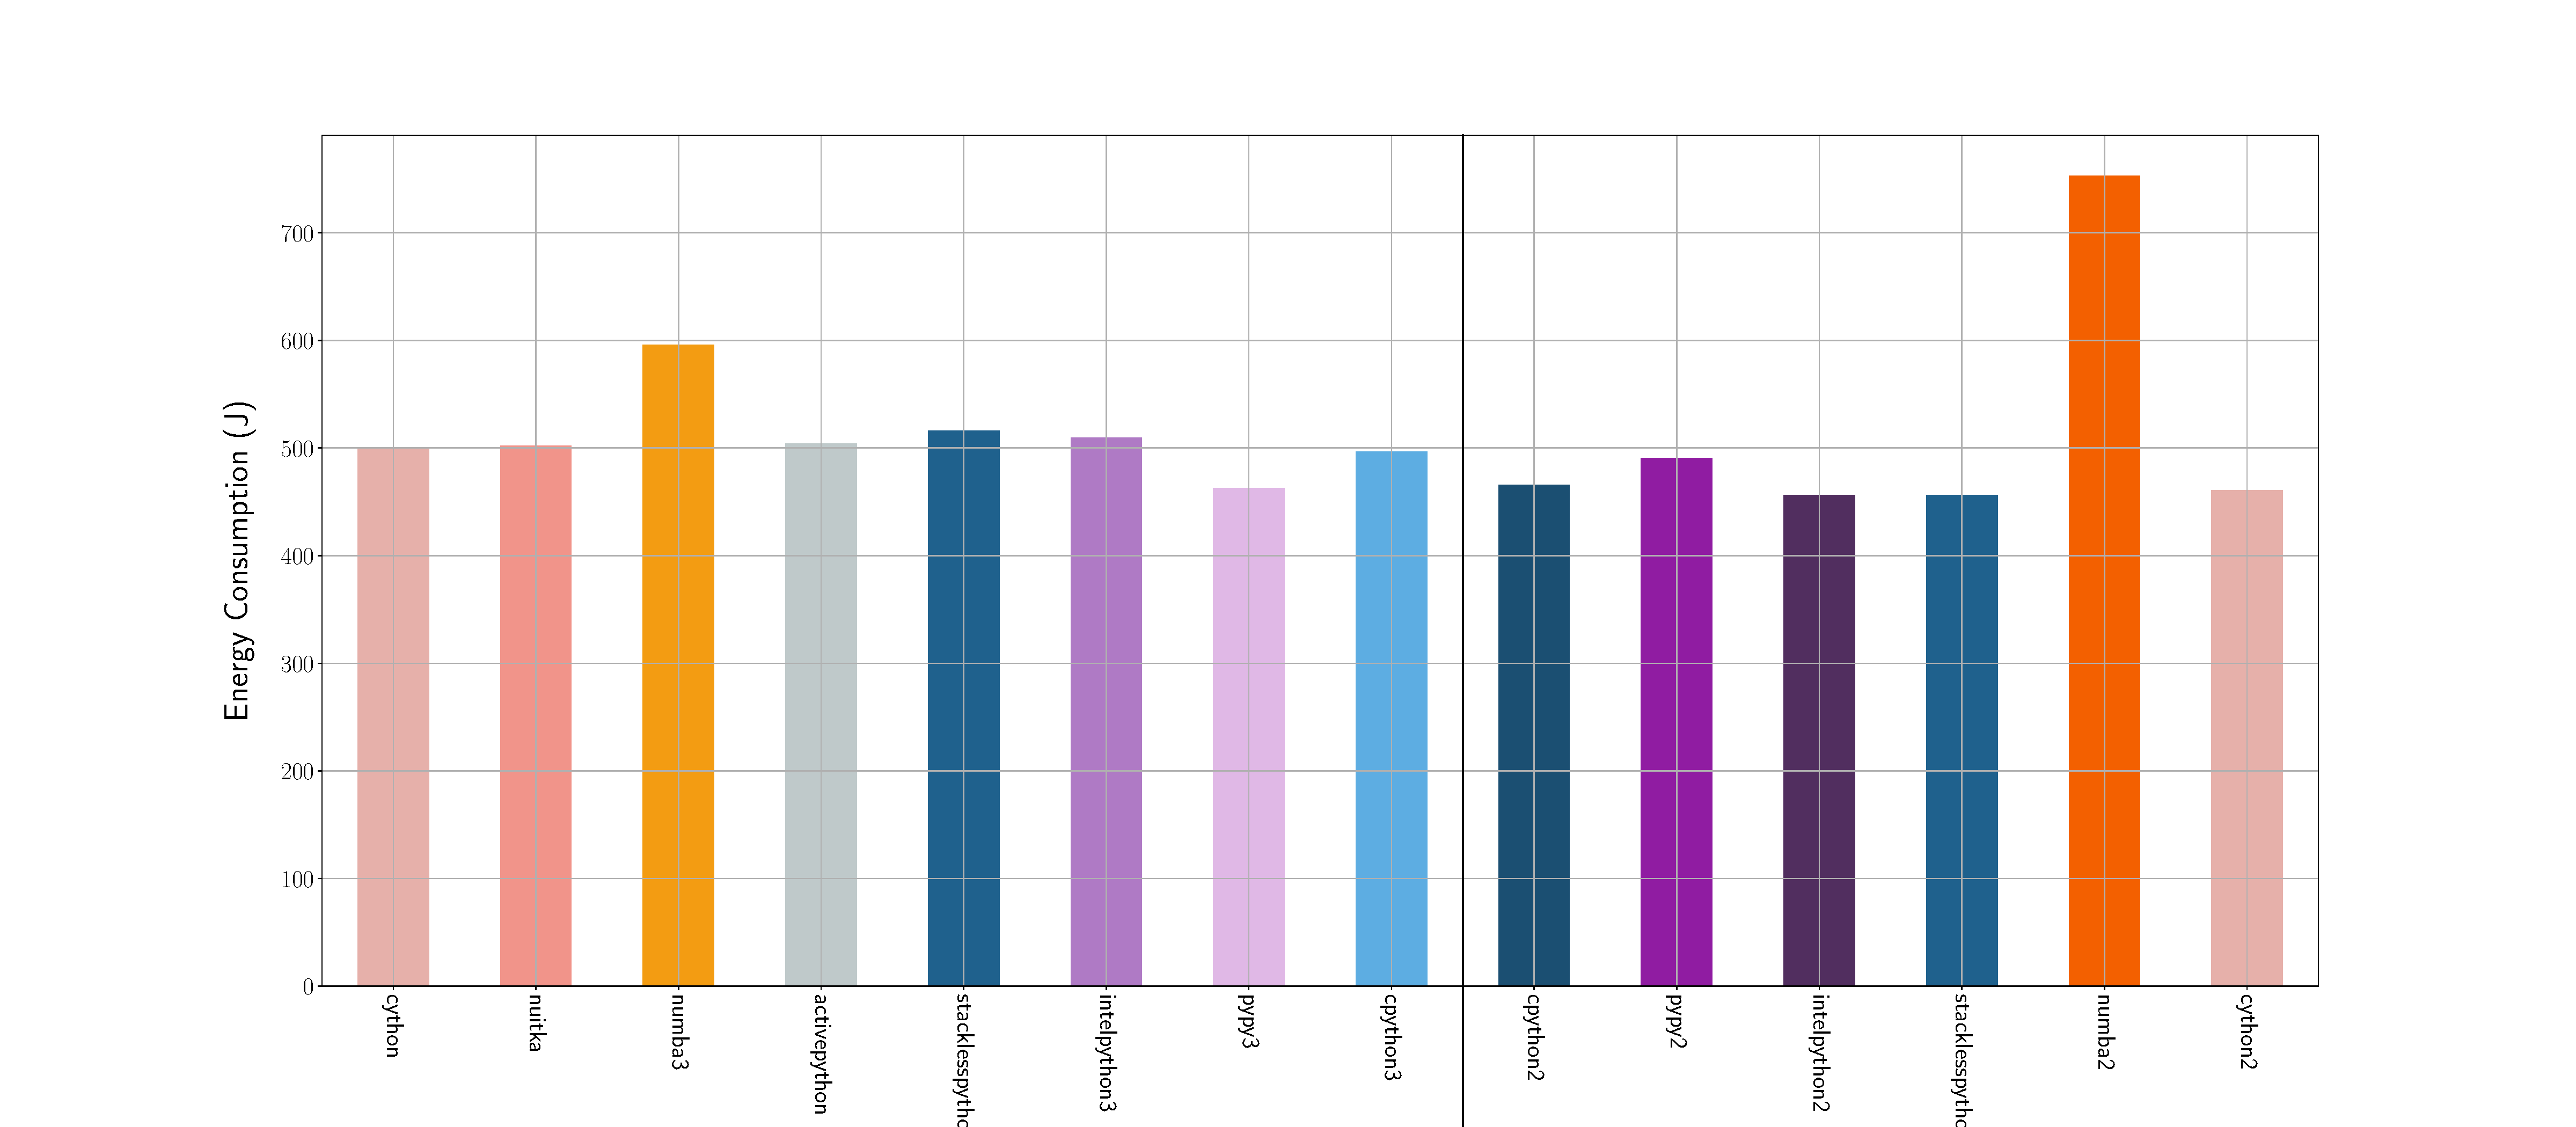
\includegraphics[width=\linewidth]{imgs/barplot_binarry_tree}
    \caption{energy behaviour based on multiprocessing}
    \label{fig:python_multiprocessing}
\end{figure}

\begin{figure}
    \centering
    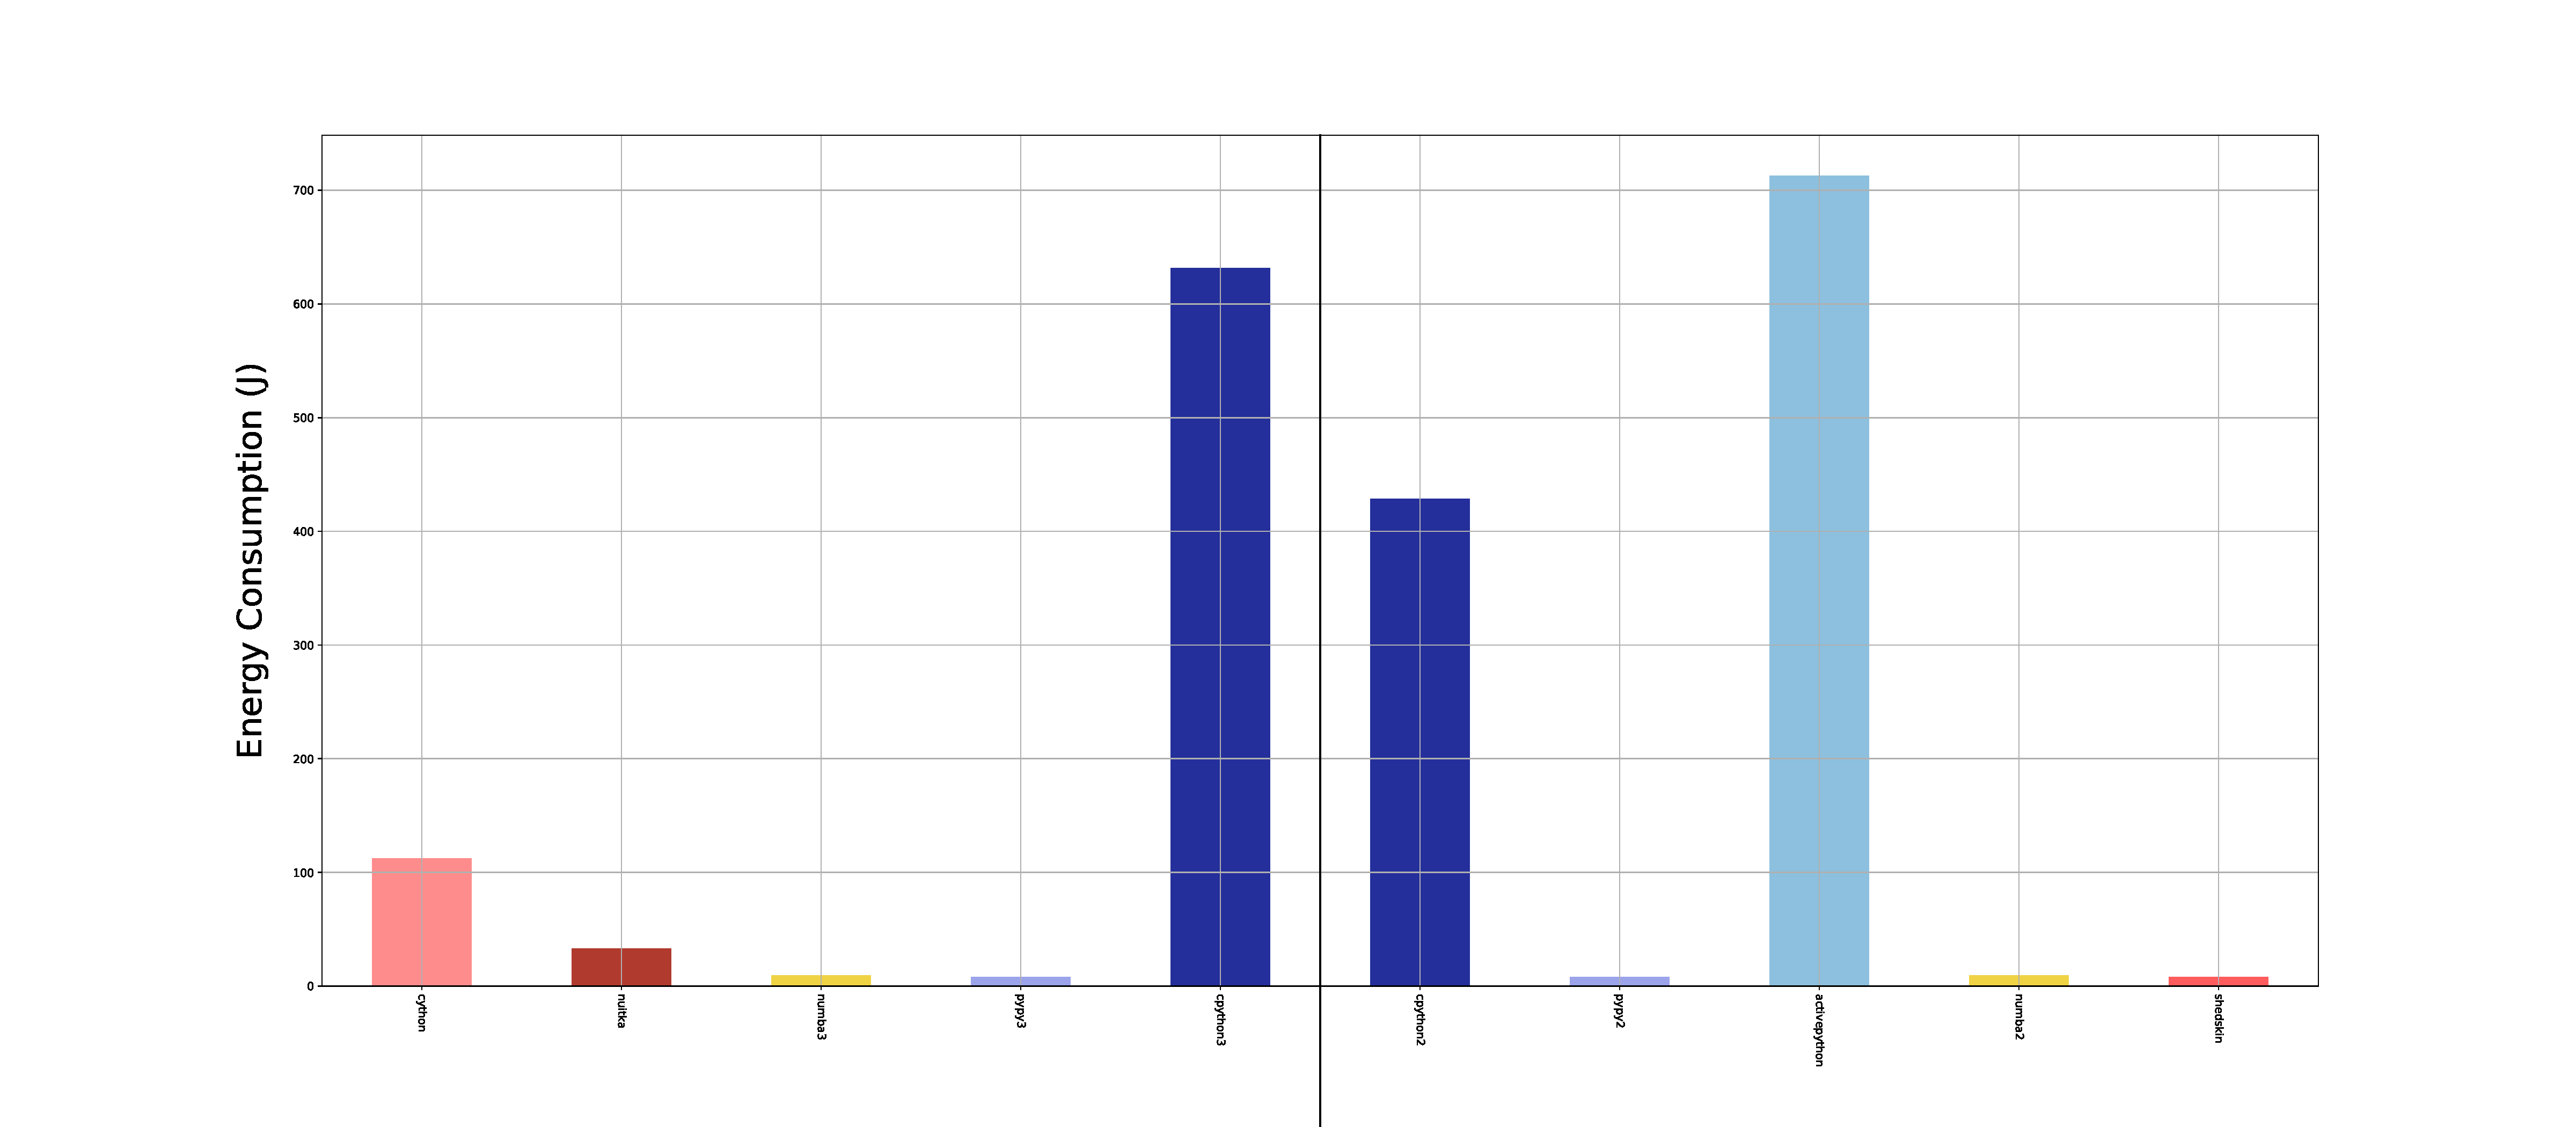
\includegraphics[width=\linewidth]{imgs/bitopts_mean}
    \caption{Mean consumption of different implementations of bit operations (Joule) }
    \label{fig:bitops}
\end{figure}

\begin{figure}
    \centering
    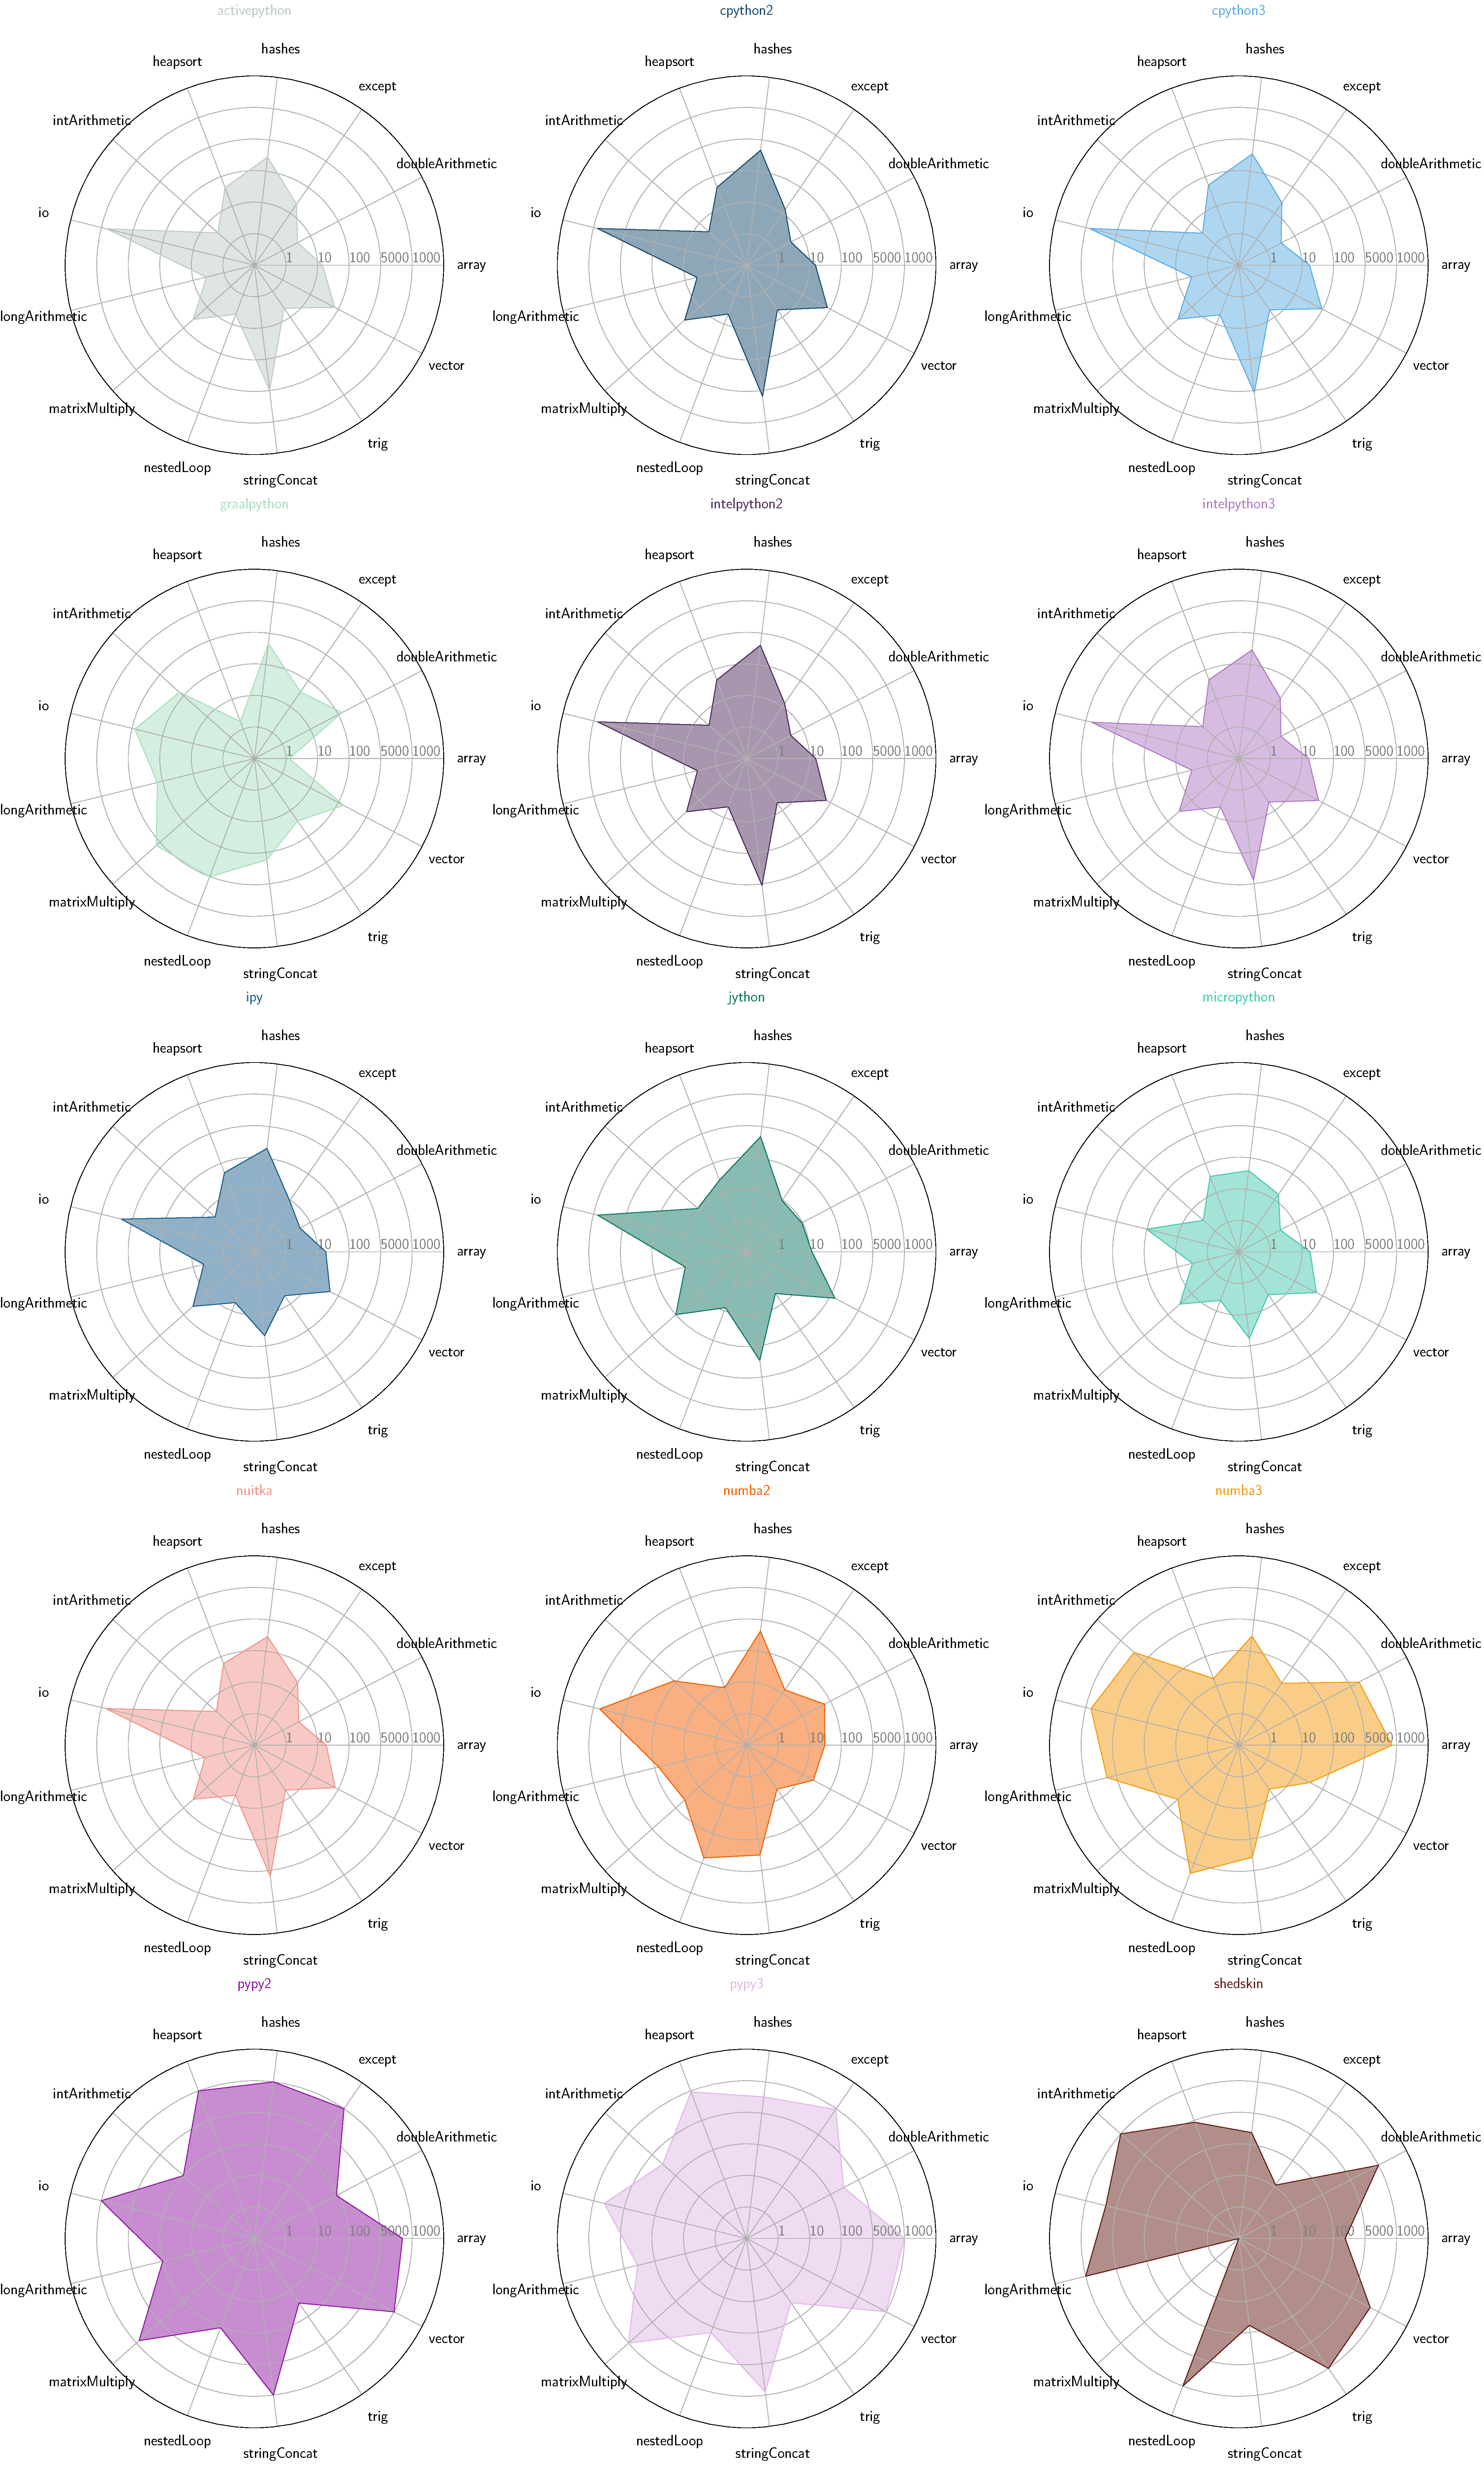
\includegraphics[width=\linewidth]{imgs/alltomti_performance}
    \caption{different interpererts optimisation }
    \label{fig:tommi_all}
\end{figure}
\begin{figure}
    \centering
    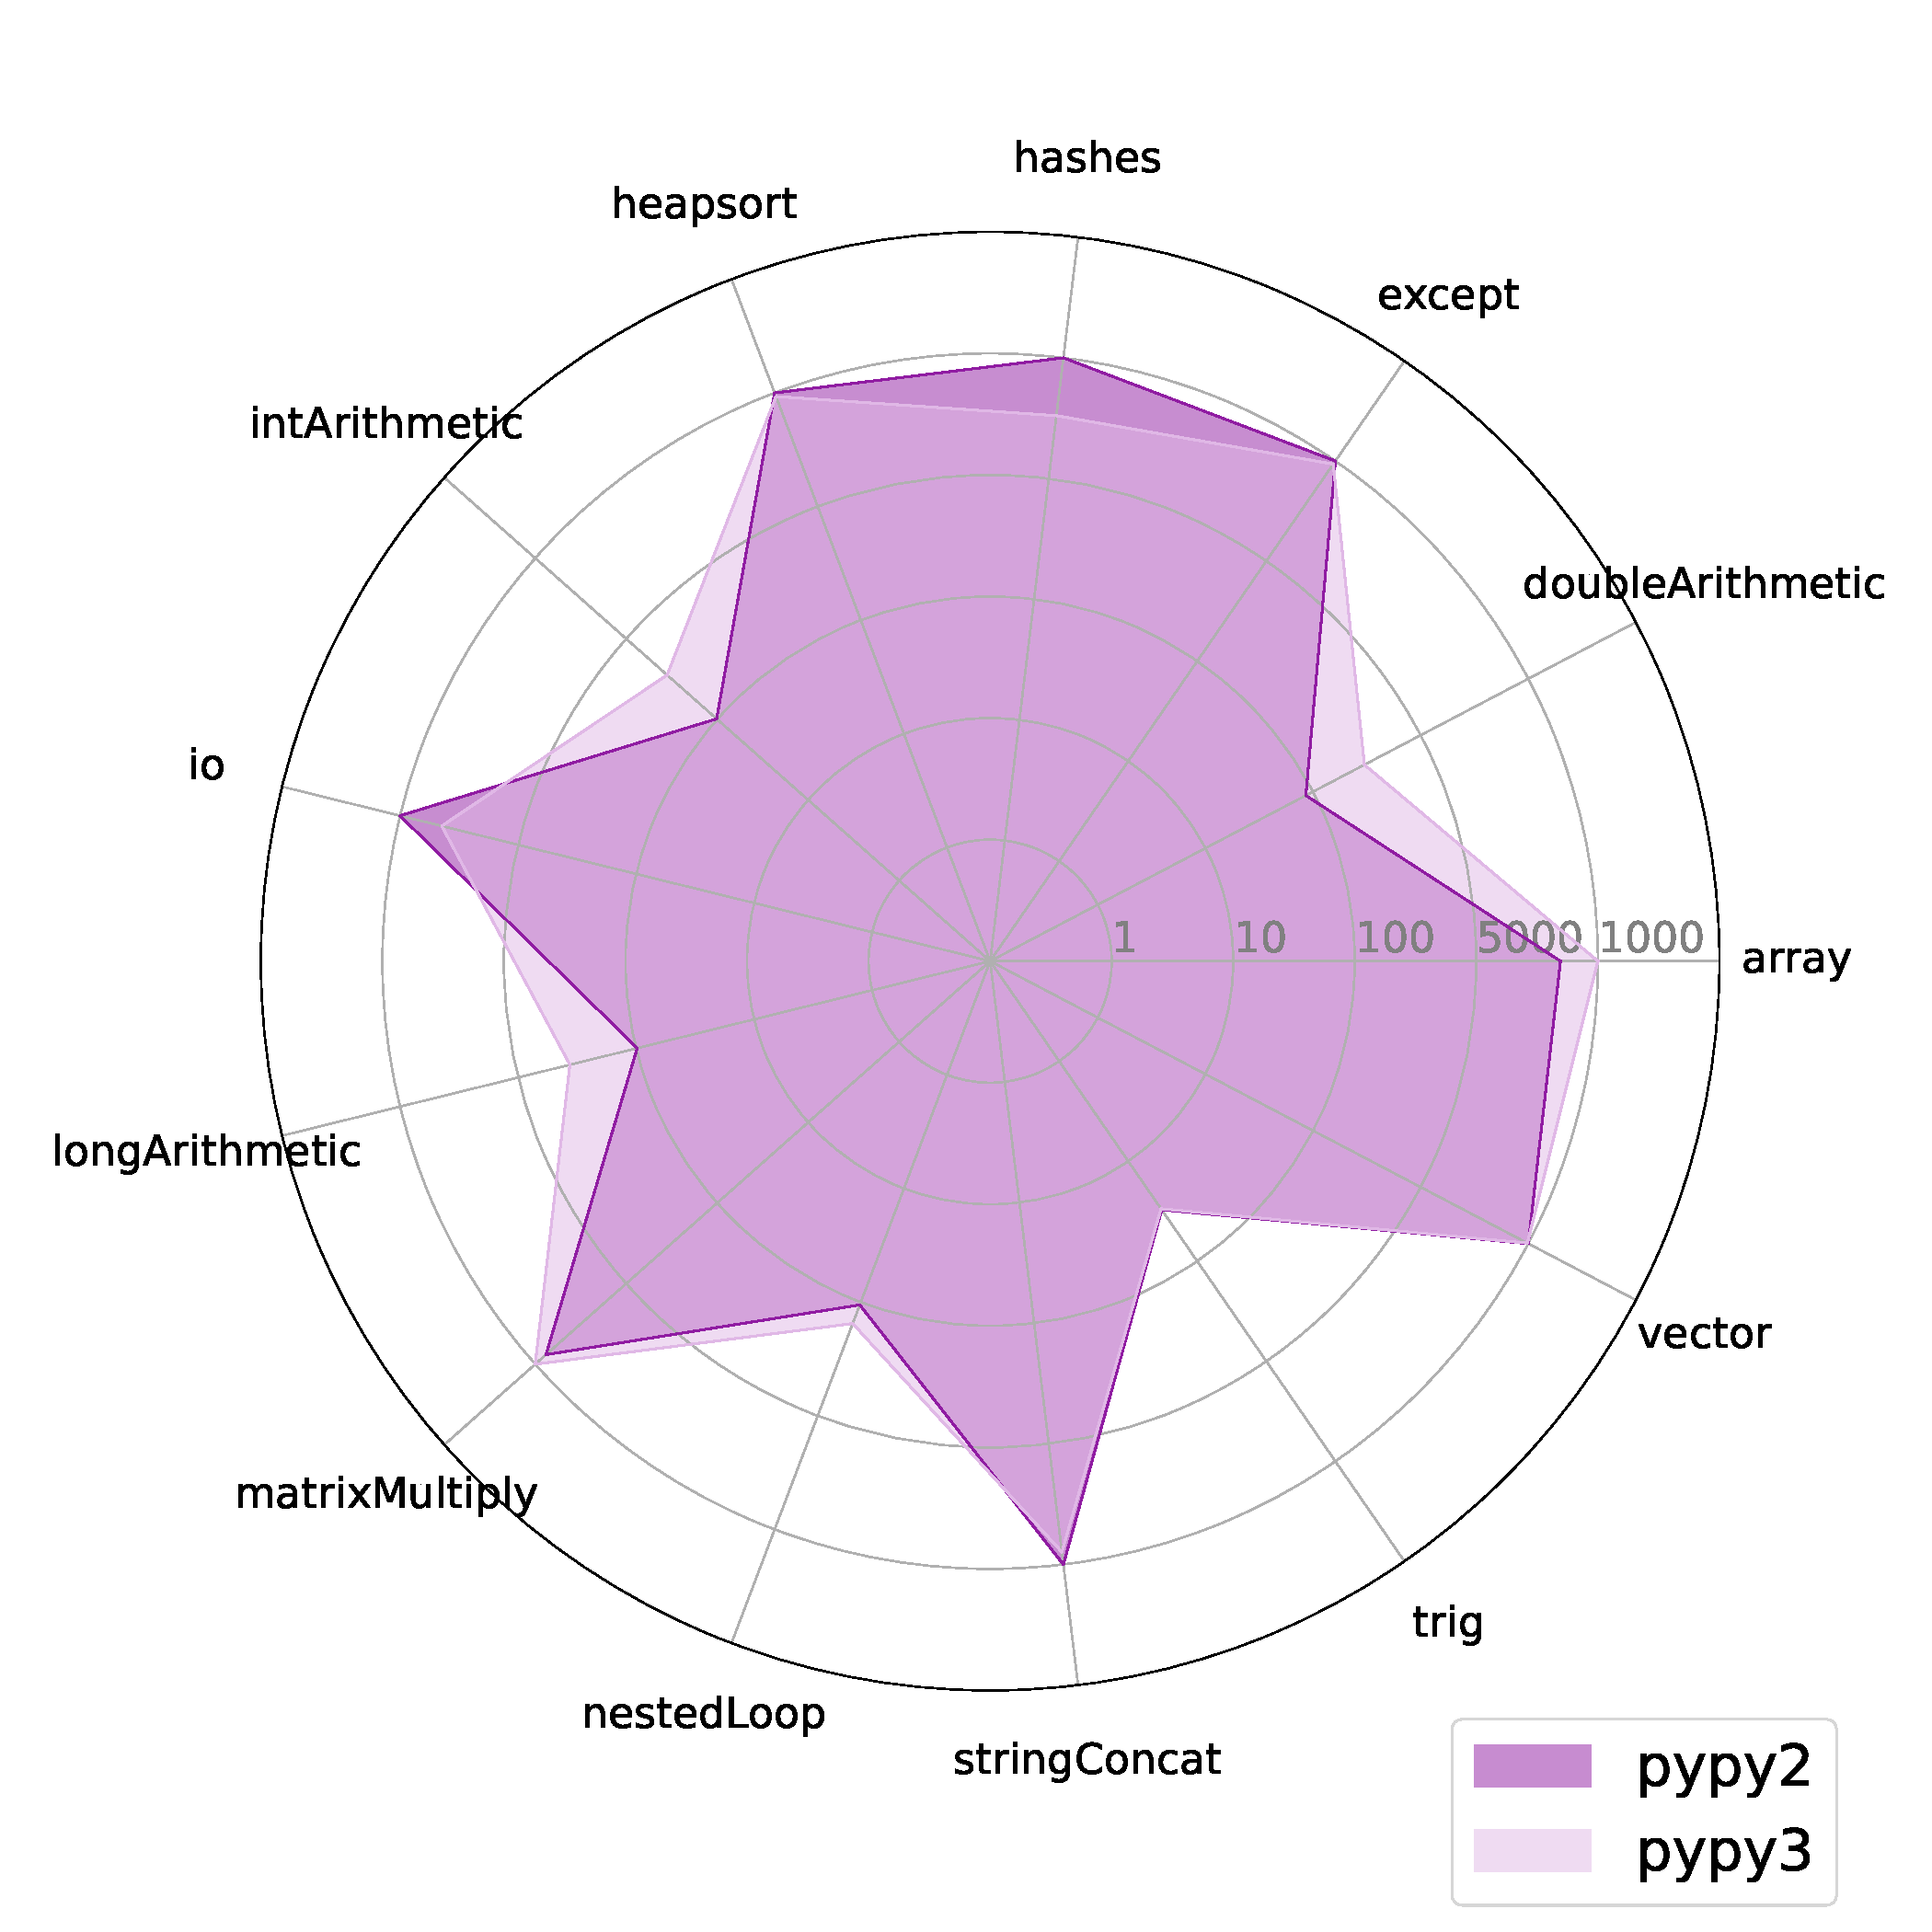
\includegraphics[width=\linewidth]{imgs/tommti_compare__pypy2_pypy3}
    \caption{green factor of pypy }
    \label{fig:pypy2vspypy3}
\end{figure}

\begin{figure}
    \centering
    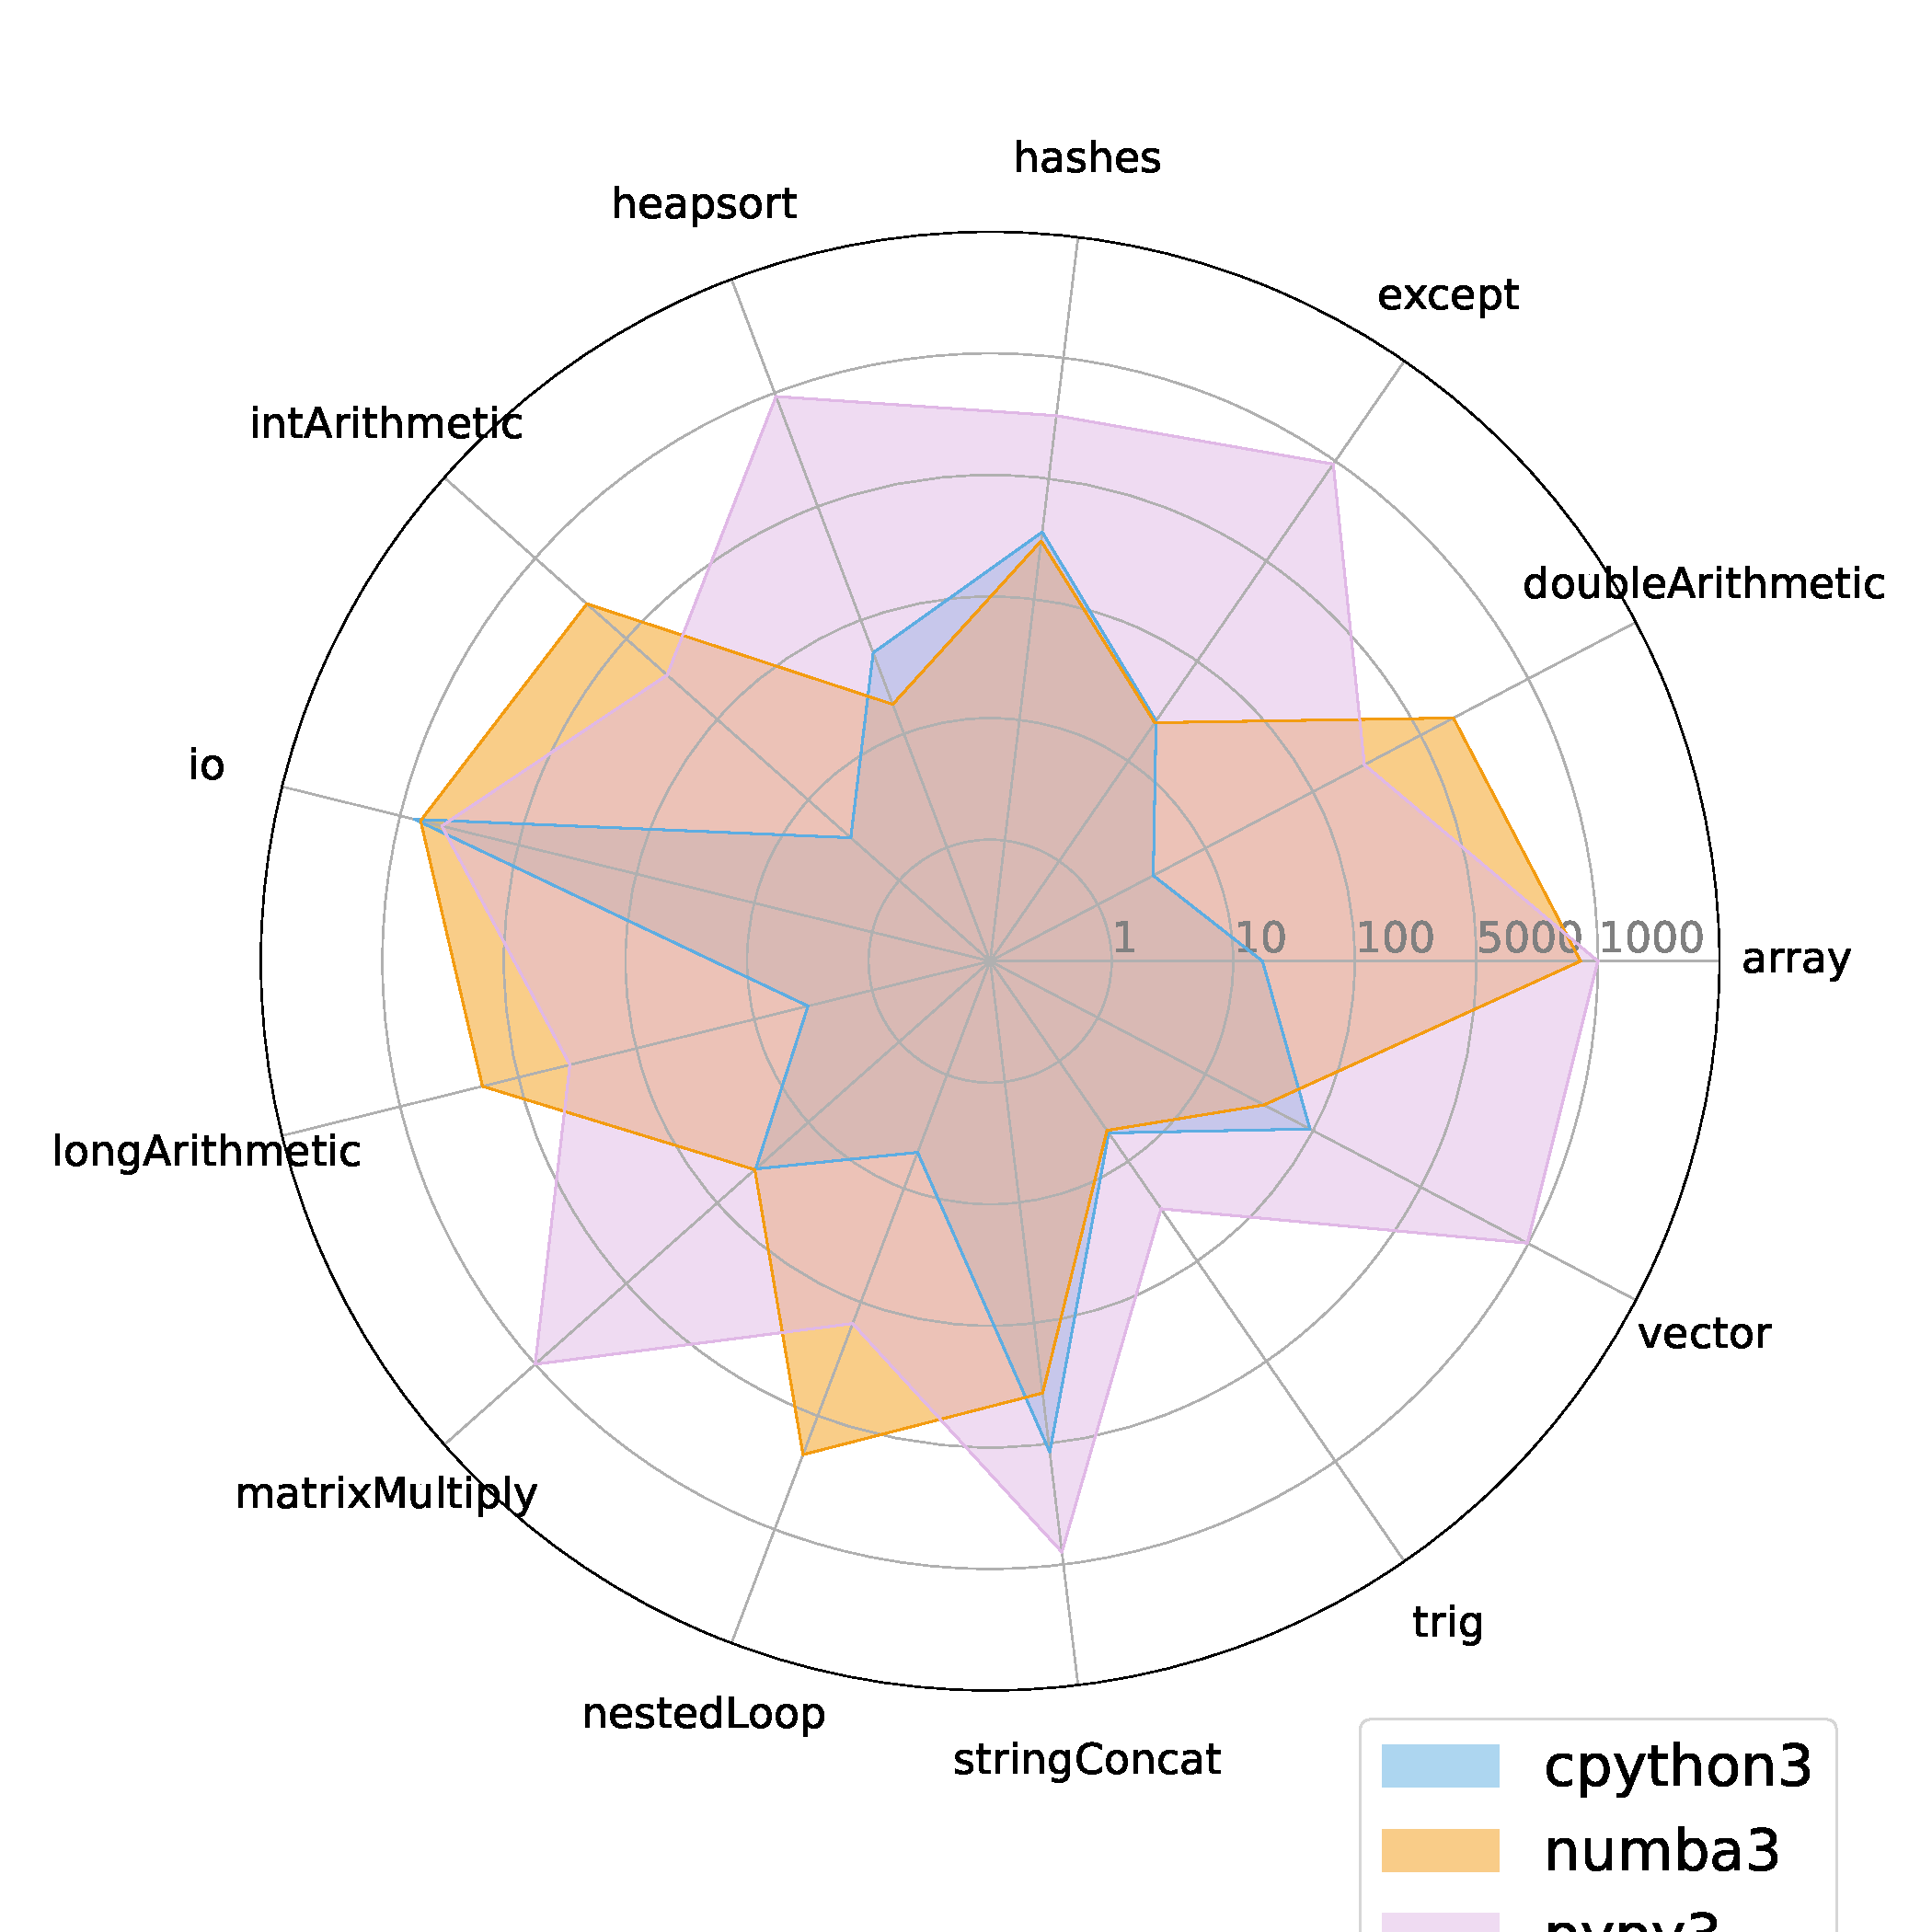
\includegraphics[width=\linewidth]{imgs/tommti_compare__cpython3_numba3_pypy3}
    \caption{comparaison of pypy vs python vs numba }
    \label{fig:p3}
\end{figure}

\begin{figure}
    \centering
    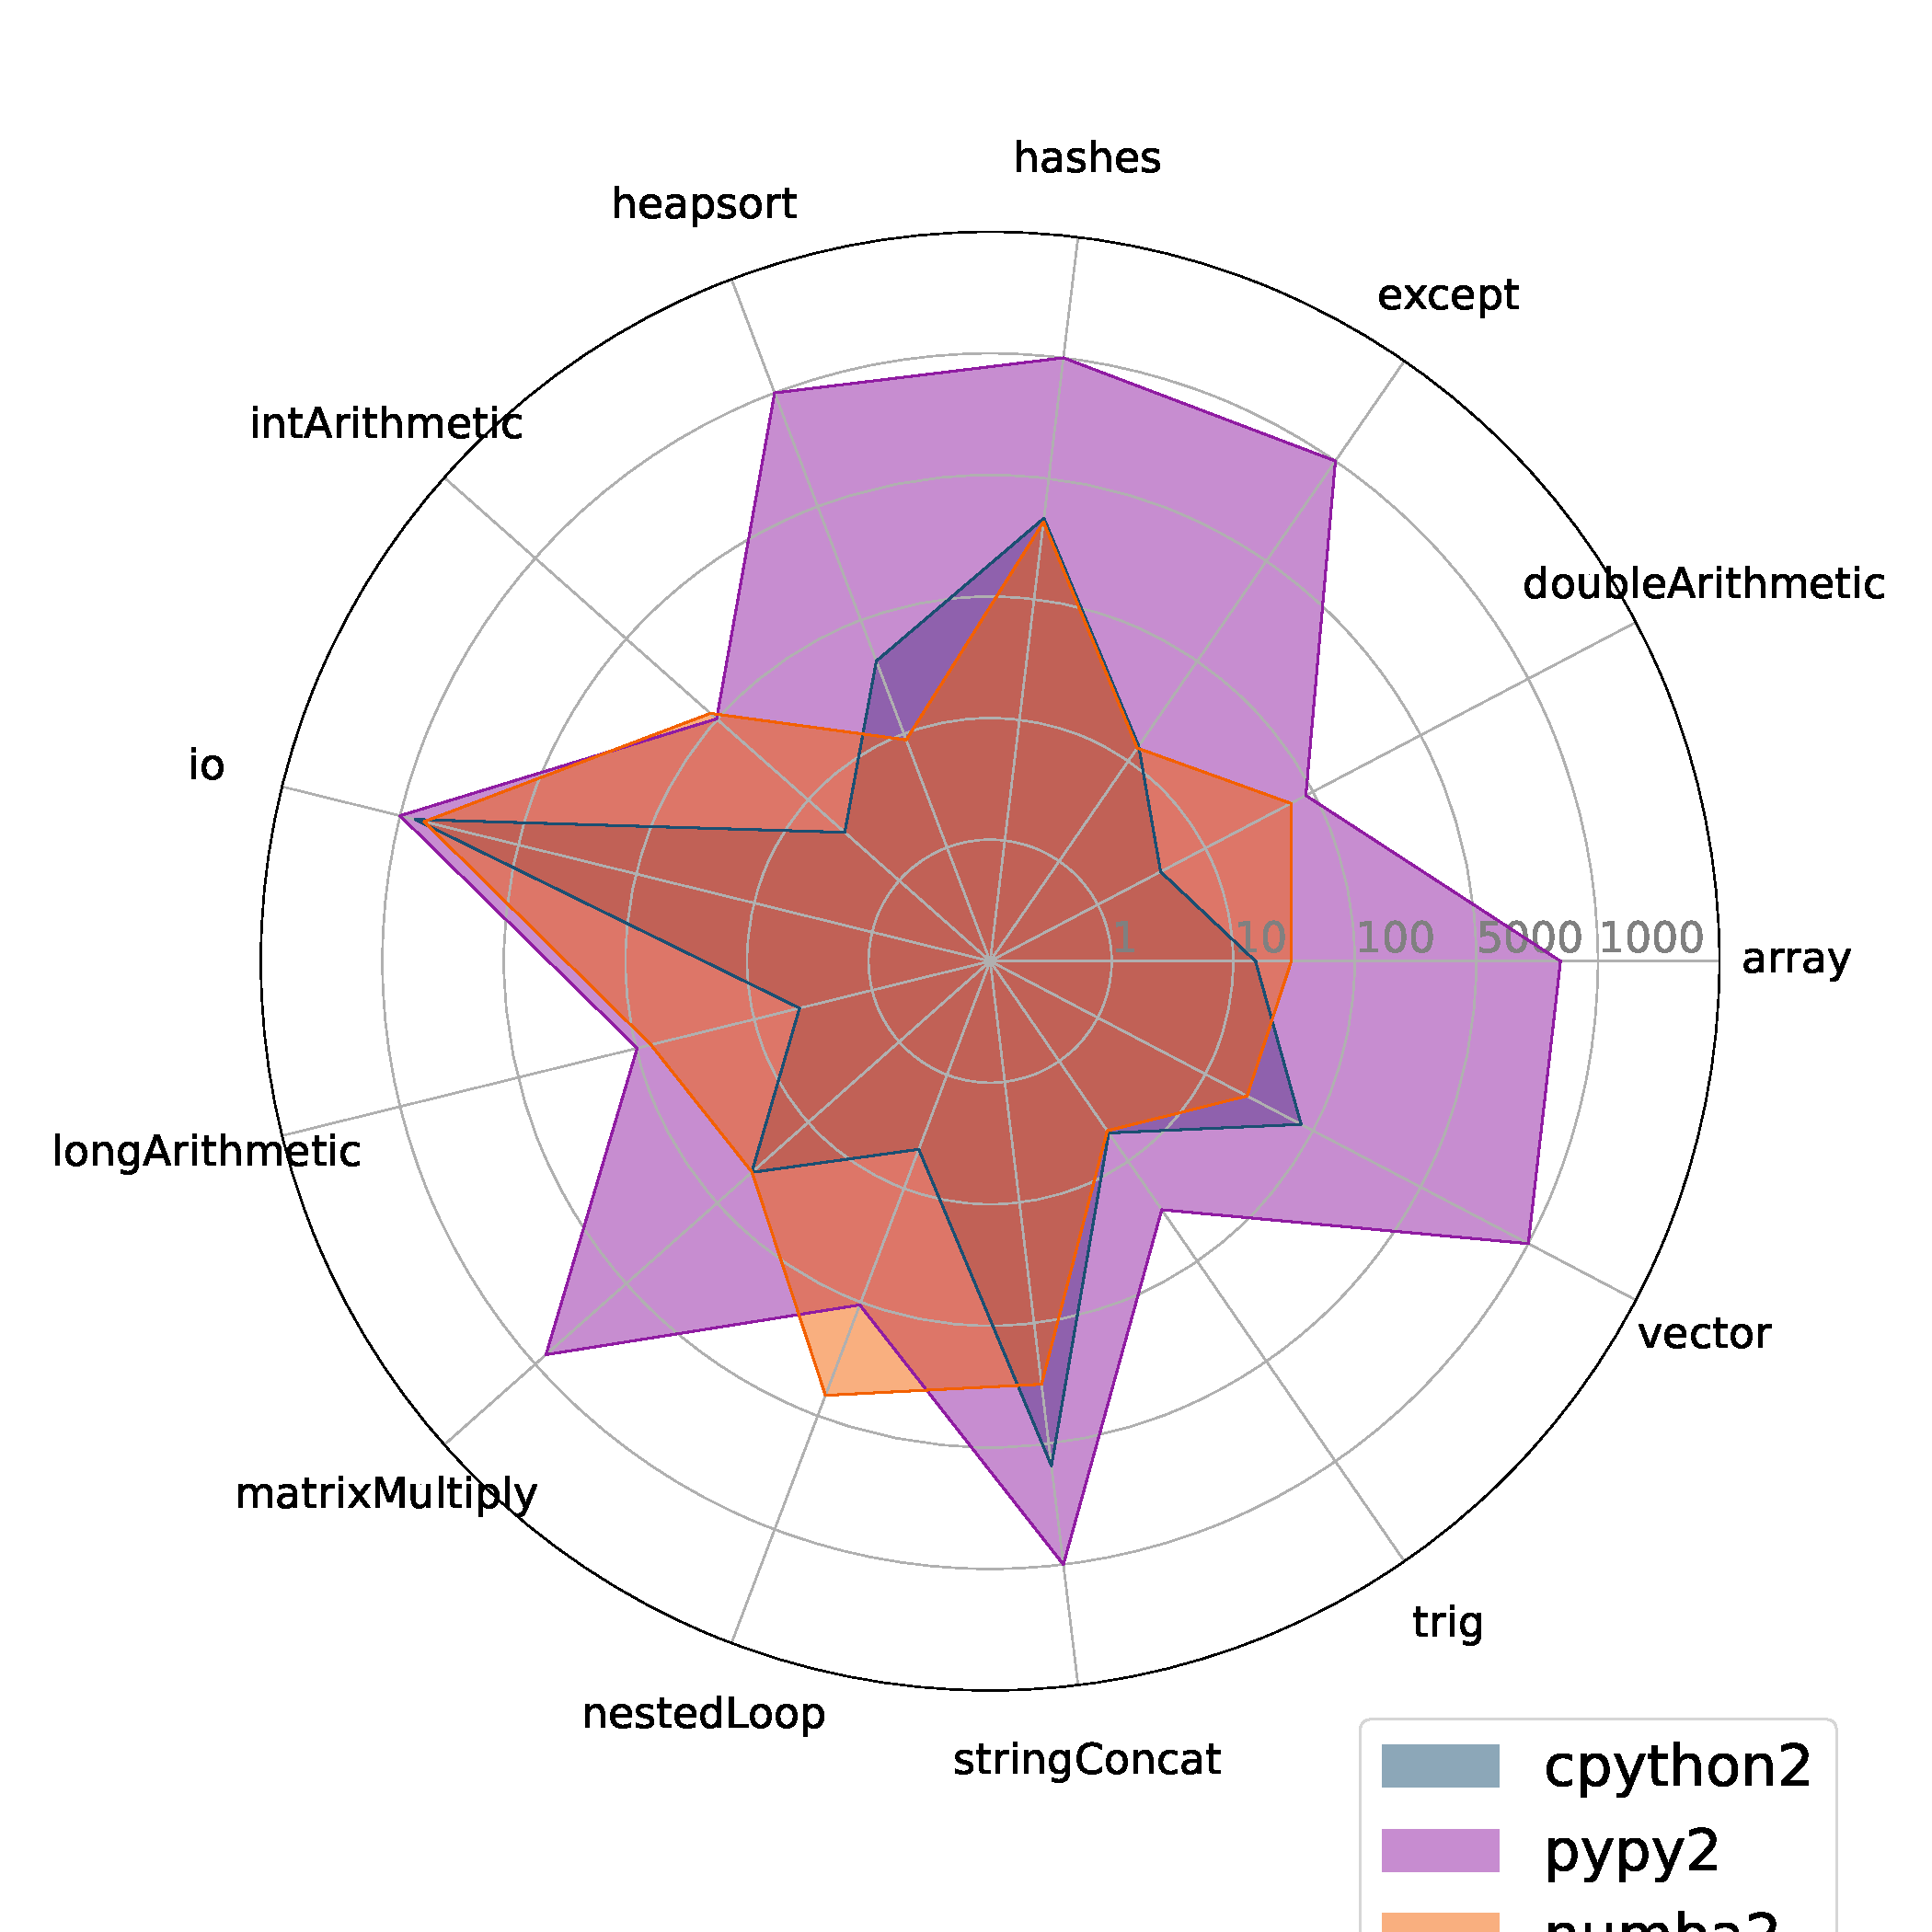
\includegraphics[width=\linewidth]{imgs/tommti_compare__cpython2_pypy2_numba2}
    \caption{comparaison of pypy vs python vs numba }
    \label{fig:p2}
\end{figure}

As we can see in figure \ref{fig:tommi_all}, there is no evolution between cpython2 and cpython3
Intelpython and active python both folows the same behaviour. one can conclude that the work that have been on those interpreters is mainly
to improve a specific purpose, Active python claims that their version is focused on secuirty which explains the lack of some performances due to the introduction of more reonforcment
.Morver Intel published their version of python as a dedicated for machine learning. Unfortunately the tommti benchmark is a set that focuses on the general purpose programming
which does not reflect the performance of the machine learning.
Another aspect of a such behaviour might be due to the fact of the processors that were used in the testbed. and it might change in the future if we include the GPU part for the machine learning benchmarks
% reference the work of the intern 
As for nuitka. there were no optimization in the energy consumpotion despite the fact that is it a complier.
However if we dig through the nuitka mechanisms. they basically embed the python code with an interpreter.
Unllike nuitka shedskin exhebit a the best energy consumption pattern when it comes to the arithmetic operartions. One can conclude it is due to the fact of the native type of the variables. unlike the interpreters where they are treated as object in the begining.

for the other interpeters pypy is very promising especially when it comes to data maniupulation as one can see in the figure \ref{fig:bar_tommti_vector}
pypy is by far the best interperer when it comes to treating vectors.
numba2 introduced the JIT but wasn't as promising as numba3.

for the other vm based interpereters. jython and ipy lacked in term of energy optimisation which was kinda expected since they were in their the begining of the stage and the main puprose of such implementation is to link the bytecode generated by jython and ironpython with their respectives virtual machin.

Unlike the the previous interpeters. graal exhebits a certin promises when it comes to complex algorithms - nested loops -
micro python is dedicated to embeded systems so lunching it is powerful cpu machines will be misleading.

Most of the interperters had the same behaviour when it comes to the input outputs. except for jython which was kinda of a anomaly probably due to the lack of the optimizations.
% pypy handles exceptions very well 


\section{conclusion}
One may observe that the choice of Python interpreter has a significant impact on the programs' energy consumption.
This investigation is made more intriguing by the absence of a universal solution.
The primary downside is the incompatibility of some of these solutions, which causes us to make concessions when we need a generic answer.


